%% template.tex
%% from
%% bare_conf.tex
%% V1.4b
%% 2015/08/26
%% by Michael Shell
%% See:
%% http://www.michaelshell.org/
%% for current contact information.
%%
%% This is a skeleton file demonstrating the use of IEEEtran.cls
%% (requires IEEEtran.cls version 1.8b or later) with an IEEE
%% conference paper.
%%
%% Support sites:
%% http://www.michaelshell.org/tex/ieeetran/
%% http://www.ctan.org/pkg/ieeetran
%% and
%% http://www.ieee.org/

%%*************************************************************************
%% Legal Notice:
%% This code is offered as-is without any warranty either expressed or
%% implied; without even the implied warranty of MERCHANTABILITY or
%% FITNESS FOR A PARTICULAR PURPOSE!
%% User assumes all risk.
%% In no event shall the IEEE or any contributor to this code be liable for
%% any damages or losses, including, but not limited to, incidental,
%% consequential, or any other damages, resulting from the use or misuse
%% of any information contained here.
%%
%% All comments are the opinions of their respective authors and are not
%% necessarily endorsed by the IEEE.
%%
%% This work is distributed under the LaTeX Project Public License (LPPL)
%% ( http://www.latex-project.org/ ) version 1.3, and may be freely used,
%% distributed and modified. A copy of the LPPL, version 1.3, is included
%% in the base LaTeX documentation of all distributions of LaTeX released
%% 2003/12/01 or later.
%% Retain all contribution notices and credits.
%% ** Modified files should be clearly indicated as such, including  **
%% ** renaming them and changing author support contact information. **
%%*************************************************************************


% *** Authors should verify (and, if needed, correct) their LaTeX system  ***
% *** with the testflow diagnostic prior to trusting their LaTeX platform ***
% *** with production work. The IEEE's font choices and paper sizes can   ***
% *** trigger bugs that do not appear when using other class files.       ***                          ***
% The testflow support page is at:
% http://www.michaelshell.org/tex/testflow/

\documentclass[conference,final,]{IEEEtran}
% Some Computer Society conferences also require the compsoc mode option,
% but others use the standard conference format.
%
% If IEEEtran.cls has not been installed into the LaTeX system files,
% manually specify the path to it like:
% \documentclass[conference]{../sty/IEEEtran}





% Some very useful LaTeX packages include:
% (uncomment the ones you want to load)


% *** MISC UTILITY PACKAGES ***
%
%\usepackage{ifpdf}
% Heiko Oberdiek's ifpdf.sty is very useful if you need conditional
% compilation based on whether the output is pdf or dvi.
% usage:
% \ifpdf
%   % pdf code
% \else
%   % dvi code
% \fi
% The latest version of ifpdf.sty can be obtained from:
% http://www.ctan.org/pkg/ifpdf
% Also, note that IEEEtran.cls V1.7 and later provides a builtin
% \ifCLASSINFOpdf conditional that works the same way.
% When switching from latex to pdflatex and vice-versa, the compiler may
% have to be run twice to clear warning/error messages.






% *** CITATION PACKAGES ***
%
%\usepackage{cite}
% cite.sty was written by Donald Arseneau
% V1.6 and later of IEEEtran pre-defines the format of the cite.sty package
% \cite{} output to follow that of the IEEE. Loading the cite package will
% result in citation numbers being automatically sorted and properly
% "compressed/ranged". e.g., [1], [9], [2], [7], [5], [6] without using
% cite.sty will become [1], [2], [5]--[7], [9] using cite.sty. cite.sty's
% \cite will automatically add leading space, if needed. Use cite.sty's
% noadjust option (cite.sty V3.8 and later) if you want to turn this off
% such as if a citation ever needs to be enclosed in parenthesis.
% cite.sty is already installed on most LaTeX systems. Be sure and use
% version 5.0 (2009-03-20) and later if using hyperref.sty.
% The latest version can be obtained at:
% http://www.ctan.org/pkg/cite
% The documentation is contained in the cite.sty file itself.






% *** GRAPHICS RELATED PACKAGES ***
%
\ifCLASSINFOpdf
  % \usepackage[pdftex]{graphicx}
  % declare the path(s) where your graphic files are
  % \graphicspath{{../pdf/}{../jpeg/}}
  % and their extensions so you won't have to specify these with
  % every instance of \includegraphics
  % \DeclareGraphicsExtensions{.pdf,.jpeg,.png}
\else
  % or other class option (dvipsone, dvipdf, if not using dvips). graphicx
  % will default to the driver specified in the system graphics.cfg if no
  % driver is specified.
  % \usepackage[dvips]{graphicx}
  % declare the path(s) where your graphic files are
  % \graphicspath{{../eps/}}
  % and their extensions so you won't have to specify these with
  % every instance of \includegraphics
  % \DeclareGraphicsExtensions{.eps}
\fi
% graphicx was written by David Carlisle and Sebastian Rahtz. It is
% required if you want graphics, photos, etc. graphicx.sty is already
% installed on most LaTeX systems. The latest version and documentation
% can be obtained at:
% http://www.ctan.org/pkg/graphicx
% Another good source of documentation is "Using Imported Graphics in
% LaTeX2e" by Keith Reckdahl which can be found at:
% http://www.ctan.org/pkg/epslatex
%
% latex, and pdflatex in dvi mode, support graphics in encapsulated
% postscript (.eps) format. pdflatex in pdf mode supports graphics
% in .pdf, .jpeg, .png and .mps (metapost) formats. Users should ensure
% that all non-photo figures use a vector format (.eps, .pdf, .mps) and
% not a bitmapped formats (.jpeg, .png). The IEEE frowns on bitmapped formats
% which can result in "jaggedy"/blurry rendering of lines and letters as
% well as large increases in file sizes.
%
% You can find documentation about the pdfTeX application at:
% http://www.tug.org/applications/pdftex





% *** MATH PACKAGES ***
%
\usepackage{amsmath}
\interdisplaylinepenalty=2500
%\usepackage{amsmath}
% A popular package from the American Mathematical Society that provides
% many useful and powerful commands for dealing with mathematics.
%
% Note that the amsmath package sets \interdisplaylinepenalty to 10000
% thus preventing page breaks from occurring within multiline equations. Use:
%\interdisplaylinepenalty=2500
% after loading amsmath to restore such page breaks as IEEEtran.cls normally
% does. amsmath.sty is already installed on most LaTeX systems. The latest
% version and documentation can be obtained at:
% http://www.ctan.org/pkg/amsmath





% *** SPECIALIZED LIST PACKAGES ***
%
%\usepackage{algorithmic}
% algorithmic.sty was written by Peter Williams and Rogerio Brito.
% This package provides an algorithmic environment fo describing algorithms.
% You can use the algorithmic environment in-text or within a figure
% environment to provide for a floating algorithm. Do NOT use the algorithm
% floating environment provided by algorithm.sty (by the same authors) or
% algorithm2e.sty (by Christophe Fiorio) as the IEEE does not use dedicated
% algorithm float types and packages that provide these will not provide
% correct IEEE style captions. The latest version and documentation of
% algorithmic.sty can be obtained at:
% http://www.ctan.org/pkg/algorithms
% Also of interest may be the (relatively newer and more customizable)
% algorithmicx.sty package by Szasz Janos:
% http://www.ctan.org/pkg/algorithmicx




% *** ALIGNMENT PACKAGES ***
%
%\usepackage{array}
% Frank Mittelbach's and David Carlisle's array.sty patches and improves
% the standard LaTeX2e array and tabular environments to provide better
% appearance and additional user controls. As the default LaTeX2e table
% generation code is lacking to the point of almost being broken with
% respect to the quality of the end results, all users are strongly
% advised to use an enhanced (at the very least that provided by array.sty)
% set of table tools. array.sty is already installed on most systems. The
% latest version and documentation can be obtained at:
% http://www.ctan.org/pkg/array


% IEEEtran contains the IEEEeqnarray family of commands that can be used to
% generate multiline equations as well as matrices, tables, etc., of high
% quality.




% *** SUBFIGURE PACKAGES ***
%\ifCLASSOPTIONcompsoc
%  \usepackage[caption=false,font=normalsize,labelfont=sf,textfont=sf]{subfig}
%\else
%  \usepackage[caption=false,font=footnotesize]{subfig}
%\fi
% subfig.sty, written by Steven Douglas Cochran, is the modern replacement
% for subfigure.sty, the latter of which is no longer maintained and is
% incompatible with some LaTeX packages including fixltx2e. However,
% subfig.sty requires and automatically loads Axel Sommerfeldt's caption.sty
% which will override IEEEtran.cls' handling of captions and this will result
% in non-IEEE style figure/table captions. To prevent this problem, be sure
% and invoke subfig.sty's "caption=false" package option (available since
% subfig.sty version 1.3, 2005/06/28) as this is will preserve IEEEtran.cls
% handling of captions.
% Note that the Computer Society format requires a larger sans serif font
% than the serif footnote size font used in traditional IEEE formatting
% and thus the need to invoke different subfig.sty package options depending
% on whether compsoc mode has been enabled.
%
% The latest version and documentation of subfig.sty can be obtained at:
% http://www.ctan.org/pkg/subfig




% *** FLOAT PACKAGES ***
%

%\usepackage{fixltx2e}
% fixltx2e, the successor to the earlier fix2col.sty, was written by
% Frank Mittelbach and David Carlisle. This package corrects a few problems
% in the LaTeX2e kernel, the most notable of which is that in current
% LaTeX2e releases, the ordering of single and double column floats is not
% guaranteed to be preserved. Thus, an unpatched LaTeX2e can allow a
% single column figure to be placed prior to an earlier double column
% figure.
% Be aware that LaTeX2e kernels dated 2015 and later have fixltx2e.sty's
% corrections already built into the system in which case a warning will
% be issued if an attempt is made to load fixltx2e.sty as it is no longer
% needed.
% The latest version and documentation can be found at:
% http://www.ctan.org/pkg/fixltx2e


%\usepackage{stfloats}
% stfloats.sty was written by Sigitas Tolusis. This package gives LaTeX2e
% the ability to do double column floats at the bottom of the page as well
% as the top. (e.g., "\begin{figure*}[!b]" is not normally possible in
% LaTeX2e). It also provides a command:
%\fnbelowfloat
% to enable the placement of footnotes below bottom floats (the standard
% LaTeX2e kernel puts them above bottom floats). This is an invasive package
% which rewrites many portions of the LaTeX2e float routines. It may not work
% with other packages that modify the LaTeX2e float routines. The latest
% version and documentation can be obtained at:
% http://www.ctan.org/pkg/stfloats
% Do not use the stfloats baselinefloat ability as the IEEE does not allow
% \baselineskip to stretch. Authors submitting work to the IEEE should note
% that the IEEE rarely uses double column equations and that authors should try
% to avoid such use. Do not be tempted to use the cuted.sty or midfloat.sty
% packages (also by Sigitas Tolusis) as the IEEE does not format its papers in
% such ways.
% Do not attempt to use stfloats with fixltx2e as they are incompatible.
% Instead, use Morten Hogholm'a dblfloatfix which combines the features
% of both fixltx2e and stfloats:
%
% \usepackage{dblfloatfix}
% The latest version can be found at:
% http://www.ctan.org/pkg/dblfloatfix




% *** PDF, URL AND HYPERLINK PACKAGES ***
%
%\usepackage{url}
% url.sty was written by Donald Arseneau. It provides better support for
% handling and breaking URLs. url.sty is already installed on most LaTeX
% systems. The latest version and documentation can be obtained at:
% http://www.ctan.org/pkg/url
% Basically, \url{my_url_here}.




% *** Do not adjust lengths that control margins, column widths, etc. ***
% *** Do not use packages that alter fonts (such as pslatex).         ***
% There should be no need to do such things with IEEEtran.cls V1.6 and later.
% (Unless specifically asked to do so by the journal or conference you plan
% to submit to, of course. )



%% BEGIN MY ADDITIONS %%



\usepackage[unicode=true]{hyperref}

\hypersetup{
            pdftitle={Feasibility study on the use of recycling materials for prototyping purposes: a comparative study based on the mechanical resistance},
            pdfkeywords={keyword 1, keyword 2},
            colorlinks=true,
            linkcolor=blue,
            citecolor=Blue,
            urlcolor=blue,
            breaklinks=true}
\urlstyle{same}  % don't use monospace font for urls

% Pandoc toggle for numbering sections (defaults to be off)
\setcounter{secnumdepth}{5}

% Pandoc syntax highlighting

% Pandoc citation processing
\newlength{\csllabelwidth}
\setlength{\csllabelwidth}{3em}
\newlength{\cslhangindent}
\setlength{\cslhangindent}{1.5em}
% for Pandoc 2.8 to 2.10.1
\newenvironment{cslreferences}%
  {}%
  {\par}
% For Pandoc 2.11+
\newenvironment{CSLReferences}[3] % #1 hanging-ident, #2 entry spacing
 {% don't indent paragraphs
  \setlength{\parindent}{0pt}
  % turn on hanging indent if param 1 is 1
  \ifodd #1 \everypar{\setlength{\hangindent}{\cslhangindent}}\ignorespaces\fi
  % set entry spacing
  \ifnum #2 > 0
  \setlength{\parskip}{#2\baselineskip}
  \fi
 }%
 {}
\usepackage{calc} % for calculating minipage widths
\newcommand{\CSLBlock}[1]{#1\hfill\break}
\newcommand{\CSLLeftMargin}[1]{\parbox[t]{\csllabelwidth}{#1}}
\newcommand{\CSLRightInline}[1]{\parbox[t]{\linewidth - \csllabelwidth}{#1}}
\newcommand{\CSLIndent}[1]{\hspace{\cslhangindent}#1}

% Pandoc header
\usepackage{caption}
\usepackage{float}
\usepackage{textcomp}
\usepackage{subcaption}
\usepackage{graphicx}
\usepackage{booktabs}
\usepackage{longtable}
\usepackage{array}
\usepackage{multirow}
\usepackage{wrapfig}
\usepackage{float}
\usepackage{colortbl}
\usepackage{pdflscape}
\usepackage{tabu}
\usepackage{threeparttable}
\usepackage{threeparttablex}
\usepackage[normalem]{ulem}
\usepackage{makecell}
\usepackage{xcolor}

\providecommand{\tightlist}{%
  \setlength{\itemsep}{0pt}\setlength{\parskip}{0pt}}

%% END MY ADDITIONS %%


\hyphenation{op-tical net-works semi-conduc-tor}

\begin{document}
%
% paper title
% Titles are generally capitalized except for words such as a, an, and, as,
% at, but, by, for, in, nor, of, on, or, the, to and up, which are usually
% not capitalized unless they are the first or last word of the title.
% Linebreaks \\ can be used within to get better formatting as desired.
% Do not put math or special symbols in the title.
\title{Feasibility study on the use of recycling materials for
prototyping purposes: a comparative study based on the mechanical
resistance}

% author names and affiliations
% use a multiple column layout for up to three different
% affiliations

\author{

%% ---- classic IEEETrans wide authors' list ----------------
 % -- end affiliation.wide
%% ----------------------------------------------------------



%% ---- classic IEEETrans one column per institution --------
 %% -- beg if/affiliation.institution-columnar
\IEEEauthorblockN{
  %% -- beg for/affiliation.institution.author
Victor M. López %% -- end for/affiliation.institution.author
}
\IEEEauthorblockA{Department of Mechanical and Mining Engineering\\
University of Jaén\\
23071 Jaén, Spain
  %% -- beg for/affiliation.institution.author
 %% -- end for/affiliation.institution.author
}
\and
\IEEEauthorblockN{
  %% -- beg for/affiliation.institution.author
Diego Carou %% -- end for/affiliation.institution.author
}
\IEEEauthorblockA{Department of Design in Engineering\\
University of Vigo\\
Ourense, Spain
  %% -- beg for/affiliation.institution.author
\\diecapor@uvigo.es
 %% -- end for/affiliation.institution.author
}
\and
\IEEEauthorblockN{
  %% -- beg for/affiliation.institution.author
Fabio A. Cruz S. %% -- end for/affiliation.institution.author
}
\IEEEauthorblockA{ERPI, F-54000\\
Université de Lorraine\\
Nancy, France
  %% -- beg for/affiliation.institution.author
 %% -- end for/affiliation.institution.author
}
 %% -- end for/affiliation.institution
 %% -- end if/affiliation.institution-columnar
%% ----------------------------------------------------------





%% ---- one column per author, classic/default IEEETrans ----
 %% -- end if/affiliation.institution-columnar
%% ----------------------------------------------------------

}

% conference papers do not typically use \thanks and this command
% is locked out in conference mode. If really needed, such as for
% the acknowledgment of grants, issue a \IEEEoverridecommandlockouts
% after \documentclass

% for over three affiliations, or if they all won't fit within the width
% of the page, use this alternative format:
%
%\author{\IEEEauthorblockN{Michael Shell\IEEEauthorrefmark{1},
%Homer Simpson\IEEEauthorrefmark{2},
%James Kirk\IEEEauthorrefmark{3},
%Montgomery Scott\IEEEauthorrefmark{3} and
%Eldon Tyrell\IEEEauthorrefmark{4}}
%\IEEEauthorblockA{\IEEEauthorrefmark{1}School of Electrical and Computer Engineering\\
%Georgia Institute of Technology,
%Atlanta, Georgia 30332--0250\\ Email: see http://www.michaelshell.org/contact.html}
%\IEEEauthorblockA{\IEEEauthorrefmark{2}Twentieth Century Fox, Springfield, USA\\
%Email: homer@thesimpsons.com}
%\IEEEauthorblockA{\IEEEauthorrefmark{3}Starfleet Academy, San Francisco, California 96678-2391\\
%Telephone: (800) 555--1212, Fax: (888) 555--1212}
%\IEEEauthorblockA{\IEEEauthorrefmark{4}Tyrell Inc., 123 Replicant Street, Los Angeles, California 90210--4321}}




% use for special paper notices
%\IEEEspecialpapernotice{(Invited Paper)}




% make the title area
\maketitle

% As a general rule, do not put math, special symbols or citations
% in the abstract
\begin{abstract}
Nowadays, sustainability is one of the major objectives for
manufacturing. The use of recycled materials can be a suitable strategy
when economic, environmental and technical feasibility are verified. 3D
printing is still a novel manufacturing process and the research on the
topic is still limited, particularly when referring to sustainability
issues. This paper attempts to evaluate the suitability of the
substitution of virgin polylactic acid (PLA) by recycled PLA. To do
that, it includes an experimental plan divided into three phases
including .. to evaluate the technical feasibility based on mechanical
resistance. The results showed that recycled PLA may be used due to the,
though slightly lower, similar mechanical resistance than that of the
virgin material. This reduction is limited to 13 \% in the worst
configuration (vertical). Besides, it was identified how the infill
density and the orientation used for printing played a major role on the
mechanical resistance, when others such as the infill pattern, printing
speed and layer height had non-significant influence.
\end{abstract}

% keywords
\begin{IEEEkeywords}
keyword 1; keyword 2
\end{IEEEkeywords}

% use for special paper notices



% make the title area
\maketitle

% no keywords

% For peer review papers, you can put extra information on the cover
% page as needed:
% \ifCLASSOPTIONpeerreview
% \begin{center} \bfseries EDICS Category: 3-BBND \end{center}
% \fi
%
% For peerreview papers, this IEEEtran command inserts a page break and
% creates the second title. It will be ignored for other modes.
\IEEEpeerreviewmaketitle


\hypertarget{introduction}{%
\section{Introduction}\label{introduction}}

Additive manufacturing (also called 3D printing) is becoming a key
technology for cross domains applications. The principle of
manufacturing objects layer-by-layer enables a higher flexibility degree
in the product design phase. The set of several technologies are pushing
forward the advantages such as customization of objects with complex
geometries and a great deal of detail, combination of different
materials, reduction of the need for assembly and high utilizations rate
of raw materials \protect\hyperlink{ref-Xiao2014}{{[}2{]}}. Thus, this
field is receiving great attention by the industrial companies and the
general public.

3D printing has developed significantly over time. A great development
is expected in sectors such as product consumption, medical products and
aerospace components \protect\hyperlink{ref-Peng2018}{{[}3{]}}. The
rapid prototyping market reached \$7.3 billion US dollars in 2018
according to Wohlers (Rodriguez-Hernández et al., 2020), which also
forecasts the market to reach 23.9 and 35.6 billion dollars by 2022 and
2024, respectively {[}Forbes2020{]}. The industry has grown from \$295
million to 5.1 billion over the past 25 years.

Nowadays, there is a need to find paths to reduce the ecological impact
of manufacturing processes and activities
\protect\hyperlink{ref-Niaki2019}{{[}4{]}}. Researchers are developing
efforts to identify opportunities of 3D printing on the circular economy
paradigm \protect\hyperlink{ref-Despeisse2016}{{[}5{]}}. Moreover, due
to the fact that plastic is one of the most used materials in the 3D
printing industry
\protect\hyperlink{ref-GonzalezHenriquez2019}{{[}6{]}}, and given their
non-biodegradable nature, it is one the most abundant type of waste
produced and their impact is well document in the different ecosystems
\protect\hyperlink{ref-Ryberg2019}{{[}7{]}}. Thus, reducing the
consumption of plastics and/or the use of the plastics already presented
in the ecosystem is of great importance for the environment.

A major literature validates the rationale for prototyping phase in
early design phases of product development coming from engineering,
human computer interaction, design thinking or software development
\protect\hyperlink{ref-Elverum2016a}{{[}8{]}}. According the prototyping
theory, different kind of prototypes are needed during the new product
development phases (eg. prototype for desirability, for feasibility, and
for viability) \protect\hyperlink{ref-Menold2017}{{[}9{]}}. Based on
that, a prototype is accomplished in terms of certain aims: (1) Model to
Link, (2) Model to Test, (3) Model to Communicate, (4) Model to Decide,
and (5) Model to Interact . The use of digital tools allows designers to
create highly flexible prototypes that enable short learning cycles at
an affordable cost. On the other hand, the use of 3D printing technology
enables the materialization aspect. Even if the printed part is
functional or non-functional, the printed part is found valuable in
design decisions \protect\hyperlink{ref-Elverum2016}{{[}10{]}}. However,
there is a gap in the literature in terms of sustainable manufacturing
using 3D printing in the early design phases
\protect\hyperlink{ref-Peng2018}{{[}3{]}}. Although the technology
offers high efficiency in the use of material, the great democratization
of this technology could cause a rebound impact due to the increasing
generation and disposal of huge amounts of waste or polluting emissions
to fabricated virgin feedstock. Particularly, in the prototyping phases.
Without a doubt, FFF's roots are linked to the rapid prototyping concept
and in the last years it has been widely adopted by industry, academia
and users to create functional objects for their designs. Therefore, one
question that remains is to define the minimal conditions and mechanical
properties in order to create prototypes in the early phases without
compromising the mechanical properties, even for recycled feedstocks.

Studies on the technical acceptability of recycled materials as
substitutes for conventional virgin materials are still limited for
particular applications. It is important to note that in most cases,
prototypes do not require excellent mechanical resistance but the
minimum to be handled to inspect and measure. Thus, the type of material
used and its amount can be further optimized when it comes to
prototyping development.

The present study evaluates the mechanical properties of both
conventional and recycled polylactic acid (PLA) materials. The objective
of the study is the assessment of the suitability of the recycled PLA as
replacement in prototyping, though its use may be further extended to
other applications. To do that, this study is based on a comprehensive
Design of Experiments (DoE) approach with three main phases in order to
evaluate the influence of several printing parameters on the mechanical
properties of the parts. In section 2, a literature review is presented
in terms of critical parameters in 3D printing technology and an
overview of the use of distributed recycling approach. Then, section 3
illustrates the methodology used in this study. In section 4, the
results of the experimental approach is presented and we concluded by a
discussion and perspectives.

\hypertarget{existing-theories-previous-work}{%
\section{Existing Theories \& Previous
Work}\label{existing-theories-previous-work}}

\hypertarget{main-parameters-on-fused-filament-fabrication}{%
\subsection{Main parameters on Fused Filament
Fabrication}\label{main-parameters-on-fused-filament-fabrication}}

One of the most common processes in 3D printing is the Fused Filament
Fabrication (FFF) (also known as fused deposition process modeling
(FDM), which is a trademark). The process is based on material
extrusion, so the material is heated above the melting point of the
material and then deposited onto a platform
\protect\hyperlink{ref-Wolszczak2018}{{[}11{]}}. In FFF/FDM, a variety
of thermoplastic materials are commonly used, such as acrylonitrile
butadiene styrene (ABS), polyvinylchloride (PVS), polycarbonate (PC),
nylon, polifenilsulfona, high density polyethylene (HDPE), low density
polyethylene (LDPE), polyethylene terephthalate (PET), high impact
polystyrene (HIPS) and polylactic acid (PLA)
\protect\hyperlink{ref-Singh2018e}{{[}14{]}}.

The mechanical properties are critical for engineering parts,
particularly, for 3D printed because of the anisotropic behaviour which
can influence up to about 47\% in the ultimate tensile strength in
function of the manufacturing parameters
\protect\hyperlink{ref-Laureto2018}{{[}15{]}}. Using a systematic
literature review, \protect\hyperlink{ref-Popescu2018}{{[}16{]}}
identified certain key parameters influencing the printed parts
including raster-to-raster air gap, raster angle, layer thickness,
infill density and build orientation.\\
Nevertheless, it is highlighted that it might be uncertain if a set of
optimal parameters for a machine/polymer/application combination can be
transferred to other 3D printers due to the issue of intra-3D printer
variability. The open source nature of the FFF development emphasizes
the need for the development of a standard experimental protocols
adequate with the features of personalization of the machines
\protect\hyperlink{ref-CruzSanchez2014}{{[}17{]}}. Therefore, it is
important to identify the most important parameters among all of the
available to carry out the process that may affect the response variable
and their expected influence based on the scientific literature
\protect\hyperlink{ref-JaisinghSheoran2019}{{[}18{]}}.

In general terms, it is found that for low values of layer height, as
well as the thickness of the deposited or printed filament, the tensile
strength of the material is improved. In addition, by orienting the
printing direction towards the direction in which the tensile load will
be applied during tensile strength, the property can be also maximized.
The importance of the printing orientation was also identified by
\protect\hyperlink{ref-Yao2019}{{[}19{]}}. According to
\protect\hyperlink{ref-Alafaghani2018}{{[}20{]}}, a higher extrusion
temperature and an optimized layer thickness, a triangular filling
pattern and a higher filling level maximize the strength of the parts.
Regarding the printing speed, it is identified that higher printing
speed with higher layer thickness leads to lower part strength. Among
others, \protect\hyperlink{ref-Altan2018}{{[}21{]}} also identified the
influence of the layer height on the mechanical resistance.

\hypertarget{materials-and-recycling}{%
\subsection{Materials and recycling}\label{materials-and-recycling}}

The development of new materials such as polymers, elastomers and
composites in engineering plays a fundamental role in the advance
sustainable manufacturing \protect\hyperlink{ref-Ashby2013}{{[}22{]}}.
The use of biopolymers of natural and renewable origin, replacing
synthetic polymers, is the cellulose, hemicellulose, lignin, starch,
alginate, chitosan and derivatives derived from them represent the most
abundant bio-based and renewable raw materials for different 3D printing
technologies. In addition, these biopolymers of natural origin include
lignocellulosic materials, seaweed materials and exoskeleton crustacean
materials \protect\hyperlink{ref-Liu2019a}{{[}23{]}}.
\protect\hyperlink{ref-Liu2019a}{{[}23{]}} reviews a wide range of
biobased printing materials with the adequate printing/solidification
approach and printed structures and potential applications.

Polylactic acid (PLA) is a type of natural biopolymer obtained from
crops such as starch or sugar cane. It is a biodegradable biopolymer
consisting of lactic acid molecules and it is one of the most used
materials in 3D printing. In addition, PLA is a sustainable alternative
that shows a range of crystallinity and mechanical properties between
polystyrene and polyethylene terephthalate
\protect\hyperlink{ref-Zhao2018a}{{[}13{]}}.

In the literature, the distributed recycling via additive manufacturing
approach (DRAM) makes an emphasis in the technical steps to reuse
plastic waste through the recycling chains for material extrusion based
3D printing \protect\hyperlink{ref-Little2020}{{[}26{]}}. Recycling
(totally or blending of virgin/reused) of raw material is a method of
special interest to contribute to manufacture in a sustainable way
\protect\hyperlink{ref-Zhao2018}{{[}27{]}}. In the DRAM methodology,
consumers have an economic incentive to recycle. This is because they
can use their waste as feedstock for a wide range of consumer products
that can be produced for a fraction of conventional costs of equivalent
products. Moreover, 3D printing is especially suited because it allows
producing parts with (almost) no waste and could reduce more than 40 \%
of the waste related to the used material, reusing 95 \% of the unused
material \protect\hyperlink{ref-Petrovic2011}{{[}28{]}}. Currently, most
of the cost of 3D printing is associated with the cost of the filament
\protect\hyperlink{ref-ref}{\textbf{ref?}}. By recycling raw materials
such as polylactic acid (PLA), the emissions of carbon dioxide can be
reduced in the transport to landfills or shipping to customers offering
environmental benefits \protect\hyperlink{ref-Santander2020}{{[}29{]}}.
The technical feasibility for recycling in laboratory conditions been
proved for PLA \protect\hyperlink{ref-CruzSanchez2017}{{[}30{]}}, ABS
\protect\hyperlink{ref-Vidakis2020}{{[}31{]}}, PET
\protect\hyperlink{ref-Zander2018}{{[}32{]}} that recycled plastics have
a similar performance to their virgin counterparts and they have even
been applied in the manufacture of high value products in some sectors
such as the automobile \protect\hyperlink{ref-Zhao2018}{{[}27{]}}.

However, it is important to evaluate the properties of the recycled
materials before substituting virgin for recycled materials. In this
sense, \protect\hyperlink{ref-Kumar2018b}{{[}24{]}} compared the
elongation at break, load at break, flow index, Young's module and
breaking stress of recycled ABS, high impact polystyrene (HIPS) and PLA.
The PLA showed the highest elongation at break along with the ABS. In
addition, the PLA had a higher breaking load and breaking stress,
although a smaller Young's modulus. Other authors such as
\protect\hyperlink{ref-Gu2016}{{[}33{]}} identified the suitability of
using recycled polypropylene instead of virgin polypropylene based on
mechanical properties. Specifically, they found that the use of fillers
(talc and glass fibre) improved the mechanical properties.
\protect\hyperlink{ref-Babagowda2018}{{[}34{]}} studied the influence of
the percentage of recycled PLA used in the filament (i.e., 10 to 50 \%)
showing that the smaller the percentage the higher the ultimate tensile
strength. \protect\hyperlink{ref-Pinho2020}{{[}35{]}} obtained higher
values of tensile stress for recycled PLA when comparing to the virgin
one.

As \protect\hyperlink{ref-Suarez2020}{{[}36{]}} pointed out, the use of
recycled materials is still uncertain because of the potential changes
in the material properties then recycling.
\protect\hyperlink{ref-Zhao2018}{{[}27{]}} studied the cycles of
printing that are able to withstand the PLA until it loses much of its
properties. Thus, they showed that PLA withstands two printing cycles,
since in a third cycle the mechanical properties and viscosity decreased
considerably. The increase in crystallinity and melting enthalpy and the
decrease of cold crystallization enthalpy are attributed to the 3D
printing process, not to the extrusion recycling process. Table 1 shows
the comparison of the properties between the virgin material and the
same material subjected to another printing cycle, being possible to
appreciate how properties such as the tensile strength and modulus are
close for the two materials. Similarly, other authors such as
\protect\hyperlink{ref-Lanzotti2019}{{[}37{]}} have proved how recycling
PLA provides comparable mechanical properties as the virgin material
only after a second recycling process.

The recycling of PLA has certain limitations because of reducing
molecular weight with its reuse, resulting in degradation and decrease
of mechanical properties. For instance, the addition of polidopamine
(PDA) on the surface allows improving these properties. Viscosity is
also reduced with each printing cycle but, it could be corrected by
adding virgin plastic \protect\hyperlink{ref-Zhao2018a}{{[}13{]}}. When
recycling, there is a decrease in the properties of the material as a
result of the presence of carbonyl groups and superficial pitting due to
thermomechanical degradation during the process of new melting process
occurring during 3D printing \protect\hyperlink{ref-Zhao2018}{{[}27{]}}.

It is found that this valuable literature is focused on the evaluation
and optimization of printed parts that seeks the best trade-offs among
parameters for a final product. On the other hand, the aim of the study
is to analyze the influence of major critical factors affecting the
mechanical properties in FFF, evaluating their impact on the mechanical
properties in 3D printing, particularly for both virgin and recycled
PLA. Thus, based on the results, it is expected to gain a better
understanding on the suitability of using recycled materials in 3D
printing and how to properly select the printing conditions to guarantee
sufficient mechanical resistance. In order to do that, an experimental
plan comprising three phases will be developed. This is a complementary
approach to the established literature on FFF.

\hypertarget{methods}{%
\section{Methods}\label{methods}}

\hypertarget{materials-and-equipment}{%
\subsection{Materials and equipment}\label{materials-and-equipment}}

The printing materials used in the study were virgin and recycled PLA
characterized by data listed in Table S1. Both materials were commercial
ones, the recycled PLA contained 10 \% of virgin PLA in the blend.

The 3D printer used to manufacture the specimens was a BQ's Witbox,
shown in Fig. 1a. The software used to generate the printing code was
the Ultimaker Cura 3.2.1. To perform the destructive test, the machine
used was the MTS Criterion 43 universal testing machine (MTS, 2020) (Fig
1b) with a maximum load of 50 kN, being the maximum load supported by
the LPS 104 cell of 10 kN. The clamping system was the Instron 2716-015
system with a maximum supported load of 30 kN. The selected strain rate
was 0.5 mm/min.

\begin{figure}

{\centering 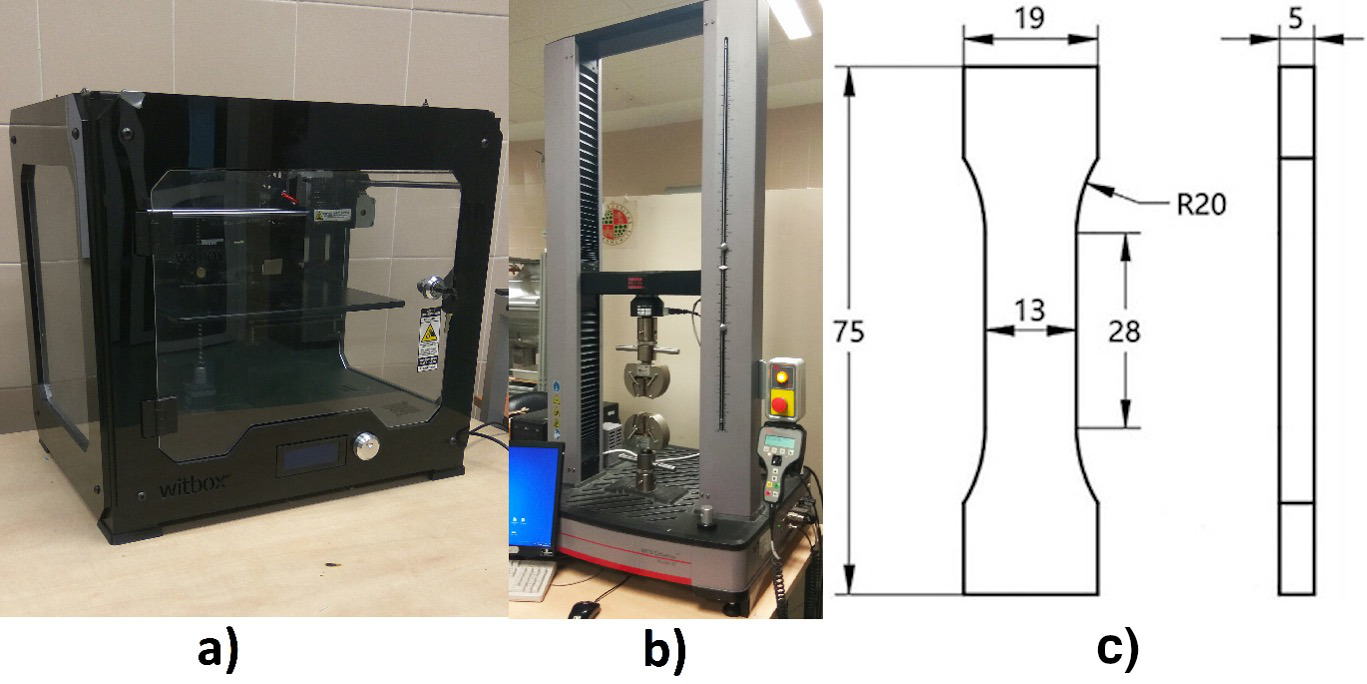
\includegraphics[width=0.9\linewidth]{Figures/Machine-probeta} 

}

\caption{Equipment used in the study: a) 3D printer, b) Universal testing machine an c) mechanical sample.}\label{fig:Fig.machine}
\end{figure}

In this study, the mechanical specimens were manufactured according to
the dimensions proposed by \protect\hyperlink{ref-Lin2018}{{[}38{]}} in
which the length of the specimen was 75 mm. The dimensions of the
specimen are the ones depicted in Fig. Fig 1c.

\hypertarget{methodology}{%
\subsection{Methodology}\label{methodology}}

Fractional designs are useful for reducing the number of tests reducing
time and money \protect\hyperlink{ref-Montgomery2001}{{[}39{]}}, being
used as screening designs. Hence, the experimental plan included three
different phases (Figure \ref{fig:methodology}) to carry out a
comprehensive study with a limited number of tests not compromising the
reliability of the results using fractional designs. The main goal of
\emph{Phase I} is to identify and discard factors depending on their
influence on the response variable. The response variable chosen was the
maximum load attained during the testing of the specimen
\protect\hyperlink{ref-Letcher2015}{{[}41{]}}. In this phase, the design
included only a specimen printed in the horizontal orientation for each
of the combinations, not evaluating the influence of the orientation.
The use of random order allowed guaranteeing that the hypothesis that
the errors are independently distributed random variables was fulfilled
\protect\hyperlink{ref-Montgomery2001}{{[}39{]}}. Based on the
literature research presented in section 2, the critical parameters for
the study are the (1) layer height and (2) infill pattern. In addition,
taking into account the goal of sustainable manufacturing (i.e., trying
to optimize the consumption of material), but also productivity (i.e.,
trying to minimize printing times), (3) infill density and (4) printing
speed were considered \protect\hyperlink{ref-Tanveer2019}{{[}43{]}}.
These four factors (layer height, infill pattern, infill density and
printing speed) were selected using two levels for each of them with
large ranges. In consequence, the factors and their levels used were:
layer height (0.15 and 0.3 mm), infill pattern (tri-hexagonal and grid)
, infill density (60 and 100 \%) and printing speed (40 and 80 mm/s).
The printing temperature chosen was 210 °C, which was the recommended
for PLA material. This phase ends with an analysis of variance (ANOVA)
in order to identify the influential factors on the response variable.

Then, the main goal of \emph{Phase II} is to study in more detail the
influence of the most influential factors according to the \emph{Phase
I}. In other words, the intent is to make a focus on how the response
variable evolves finding minimal and maximal values. For that reason, in
this phase an extension of the factor levels was established. On the
other hand, the criteria selection of levels for the other three factors
aimed at minimizing the printing time.

Finally, the \emph{Phase III} aimed at evaluating the influence of the
anisotropy of the specimens depending on the printing orientation, which
may notably affect the mechanical resistance of the specimen. In this
phase, the main focus is to analyse the influence of the building
orientation. Because of the anisotropy, the UNE 116005:2012 (UNE, 2012)
standard requires printing specimens in three different orientations:
edgewise (E), horizontal (H) and vertical (V), testing five samples in
each orientation. This phase included the printing of 15 specimens of
each virgin and recycled PLA.

\begin{figure}

{\centering 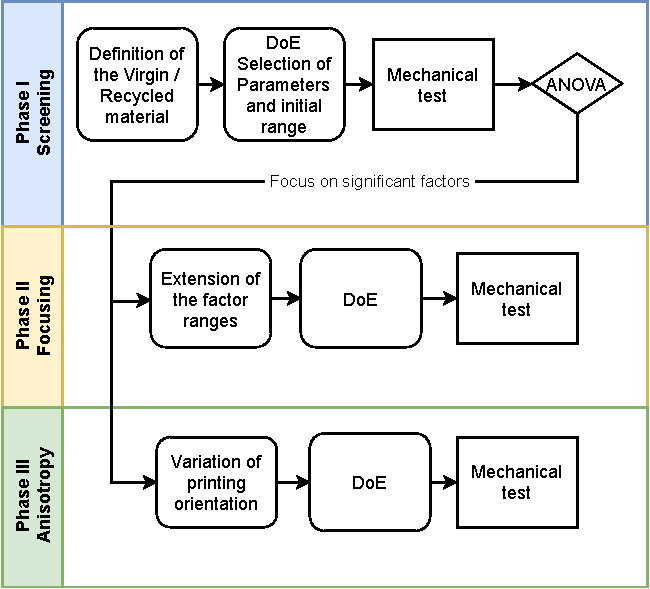
\includegraphics[width=0.8\linewidth]{Figures/Methodology} 

}

\caption{Summary of the three phases of the experimental plan.\label{fig:methodology}}\label{fig:Fig.Methodology}
\end{figure}

\hypertarget{findings}{%
\section{Findings}\label{findings}}

\hypertarget{phase-i-screening-phase}{%
\subsection{Phase I: Screening phase}\label{phase-i-screening-phase}}

Table \ref{table.phase1} summarizes the experimental strategy with the
results of the maximum load attained during this screening phase. A
total of 16 samples were tested.

\begin{table}

\caption{\label{tab:table.S2}Results of the Phase 1. \label{tab:anova.phase1}}
\centering
\begin{threeparttable}
\begin{tabular}[t]{lllrrr}
\toprule
Material & LH & IP & ID & PS & Load.max\\
\midrule
\cellcolor{gray!6}{Virgin} & \cellcolor{gray!6}{0.15} & \cellcolor{gray!6}{Tri-hex} & \cellcolor{gray!6}{60} & \cellcolor{gray!6}{40} & \cellcolor{gray!6}{2.206}\\
Virgin & 0.3 & Tri-hex & 60 & 80 & 2.163\\
\cellcolor{gray!6}{Virgin} & \cellcolor{gray!6}{0.15} & \cellcolor{gray!6}{Grid} & \cellcolor{gray!6}{60} & \cellcolor{gray!6}{80} & \cellcolor{gray!6}{2.240}\\
Virgin & 0.3 & Grid & 100 & 80 & 3.598\\
\cellcolor{gray!6}{Virgin} & \cellcolor{gray!6}{0.3} & \cellcolor{gray!6}{Tri-hex} & \cellcolor{gray!6}{100} & \cellcolor{gray!6}{40} & \cellcolor{gray!6}{3.620}\\
Virgin & 0.15 & Tri-hex & 100 & 80 & 3.811\\
\cellcolor{gray!6}{Virgin} & \cellcolor{gray!6}{0.15} & \cellcolor{gray!6}{Grid} & \cellcolor{gray!6}{100} & \cellcolor{gray!6}{40} & \cellcolor{gray!6}{3.793}\\
Virgin & 0.3 & Grid & 60 & 40 & 2.160\\
\cellcolor{gray!6}{Recycled} & \cellcolor{gray!6}{0.15} & \cellcolor{gray!6}{Tri-hex} & \cellcolor{gray!6}{60} & \cellcolor{gray!6}{40} & \cellcolor{gray!6}{2.163}\\
Recycled & 0.3 & Tri-hex & 60 & 80 & 2.163\\
\cellcolor{gray!6}{Recycled} & \cellcolor{gray!6}{0.3} & \cellcolor{gray!6}{Grid} & \cellcolor{gray!6}{60} & \cellcolor{gray!6}{40} & \cellcolor{gray!6}{2.152}\\
Recycled & 0.15 & Tri-hex & 100 & 80 & 3.379\\
\cellcolor{gray!6}{Recycled} & \cellcolor{gray!6}{0.3} & \cellcolor{gray!6}{Tri-hex} & \cellcolor{gray!6}{100} & \cellcolor{gray!6}{40} & \cellcolor{gray!6}{3.370}\\
Recycled & 0.15 & Grid & 60 & 80 & 2.051\\
\cellcolor{gray!6}{Recycled} & \cellcolor{gray!6}{0.15} & \cellcolor{gray!6}{Grid} & \cellcolor{gray!6}{100} & \cellcolor{gray!6}{40} & \cellcolor{gray!6}{3.525}\\
Recycled & 0.3 & Grid & 100 & 80 & 3.488\\
\bottomrule
\end{tabular}
\begin{tablenotes}
\item \textit{Note: } 
\item Layer height (LH), Infill pattern (IP), Infill density (ID), Printing speed (PS)
\end{tablenotes}
\end{threeparttable}
\end{table}

\begin{figure*}[!t]
\centering
\subfloat[Tensile sample of the Phase 1]{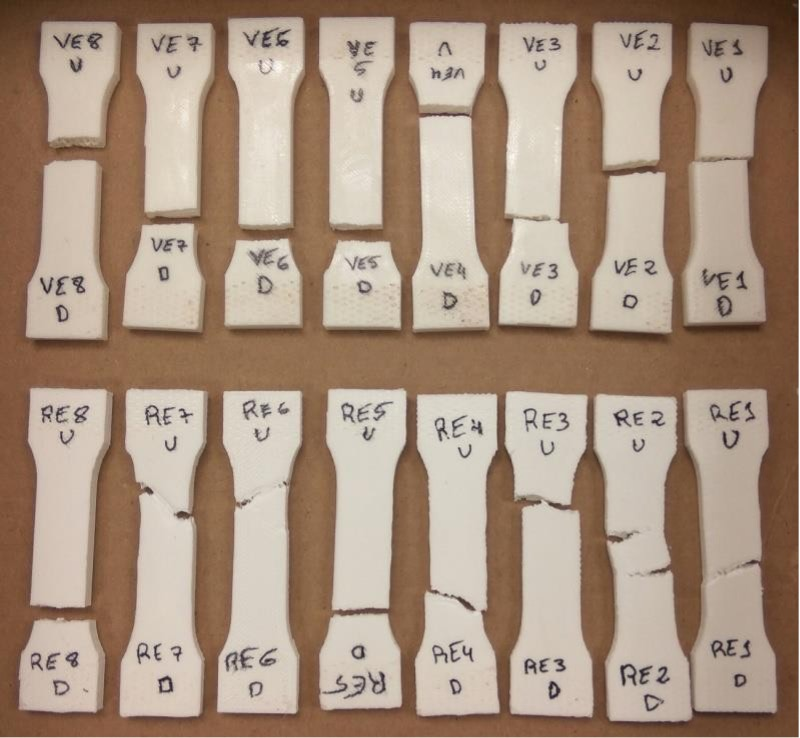
\includegraphics[width=0.4\linewidth]{Figures/Probetas-Fase-1.jpg}%
\label{Fig:Phase.1a}}
\hfil
\subfloat[Boxplots to identify significant factors based on DoE]{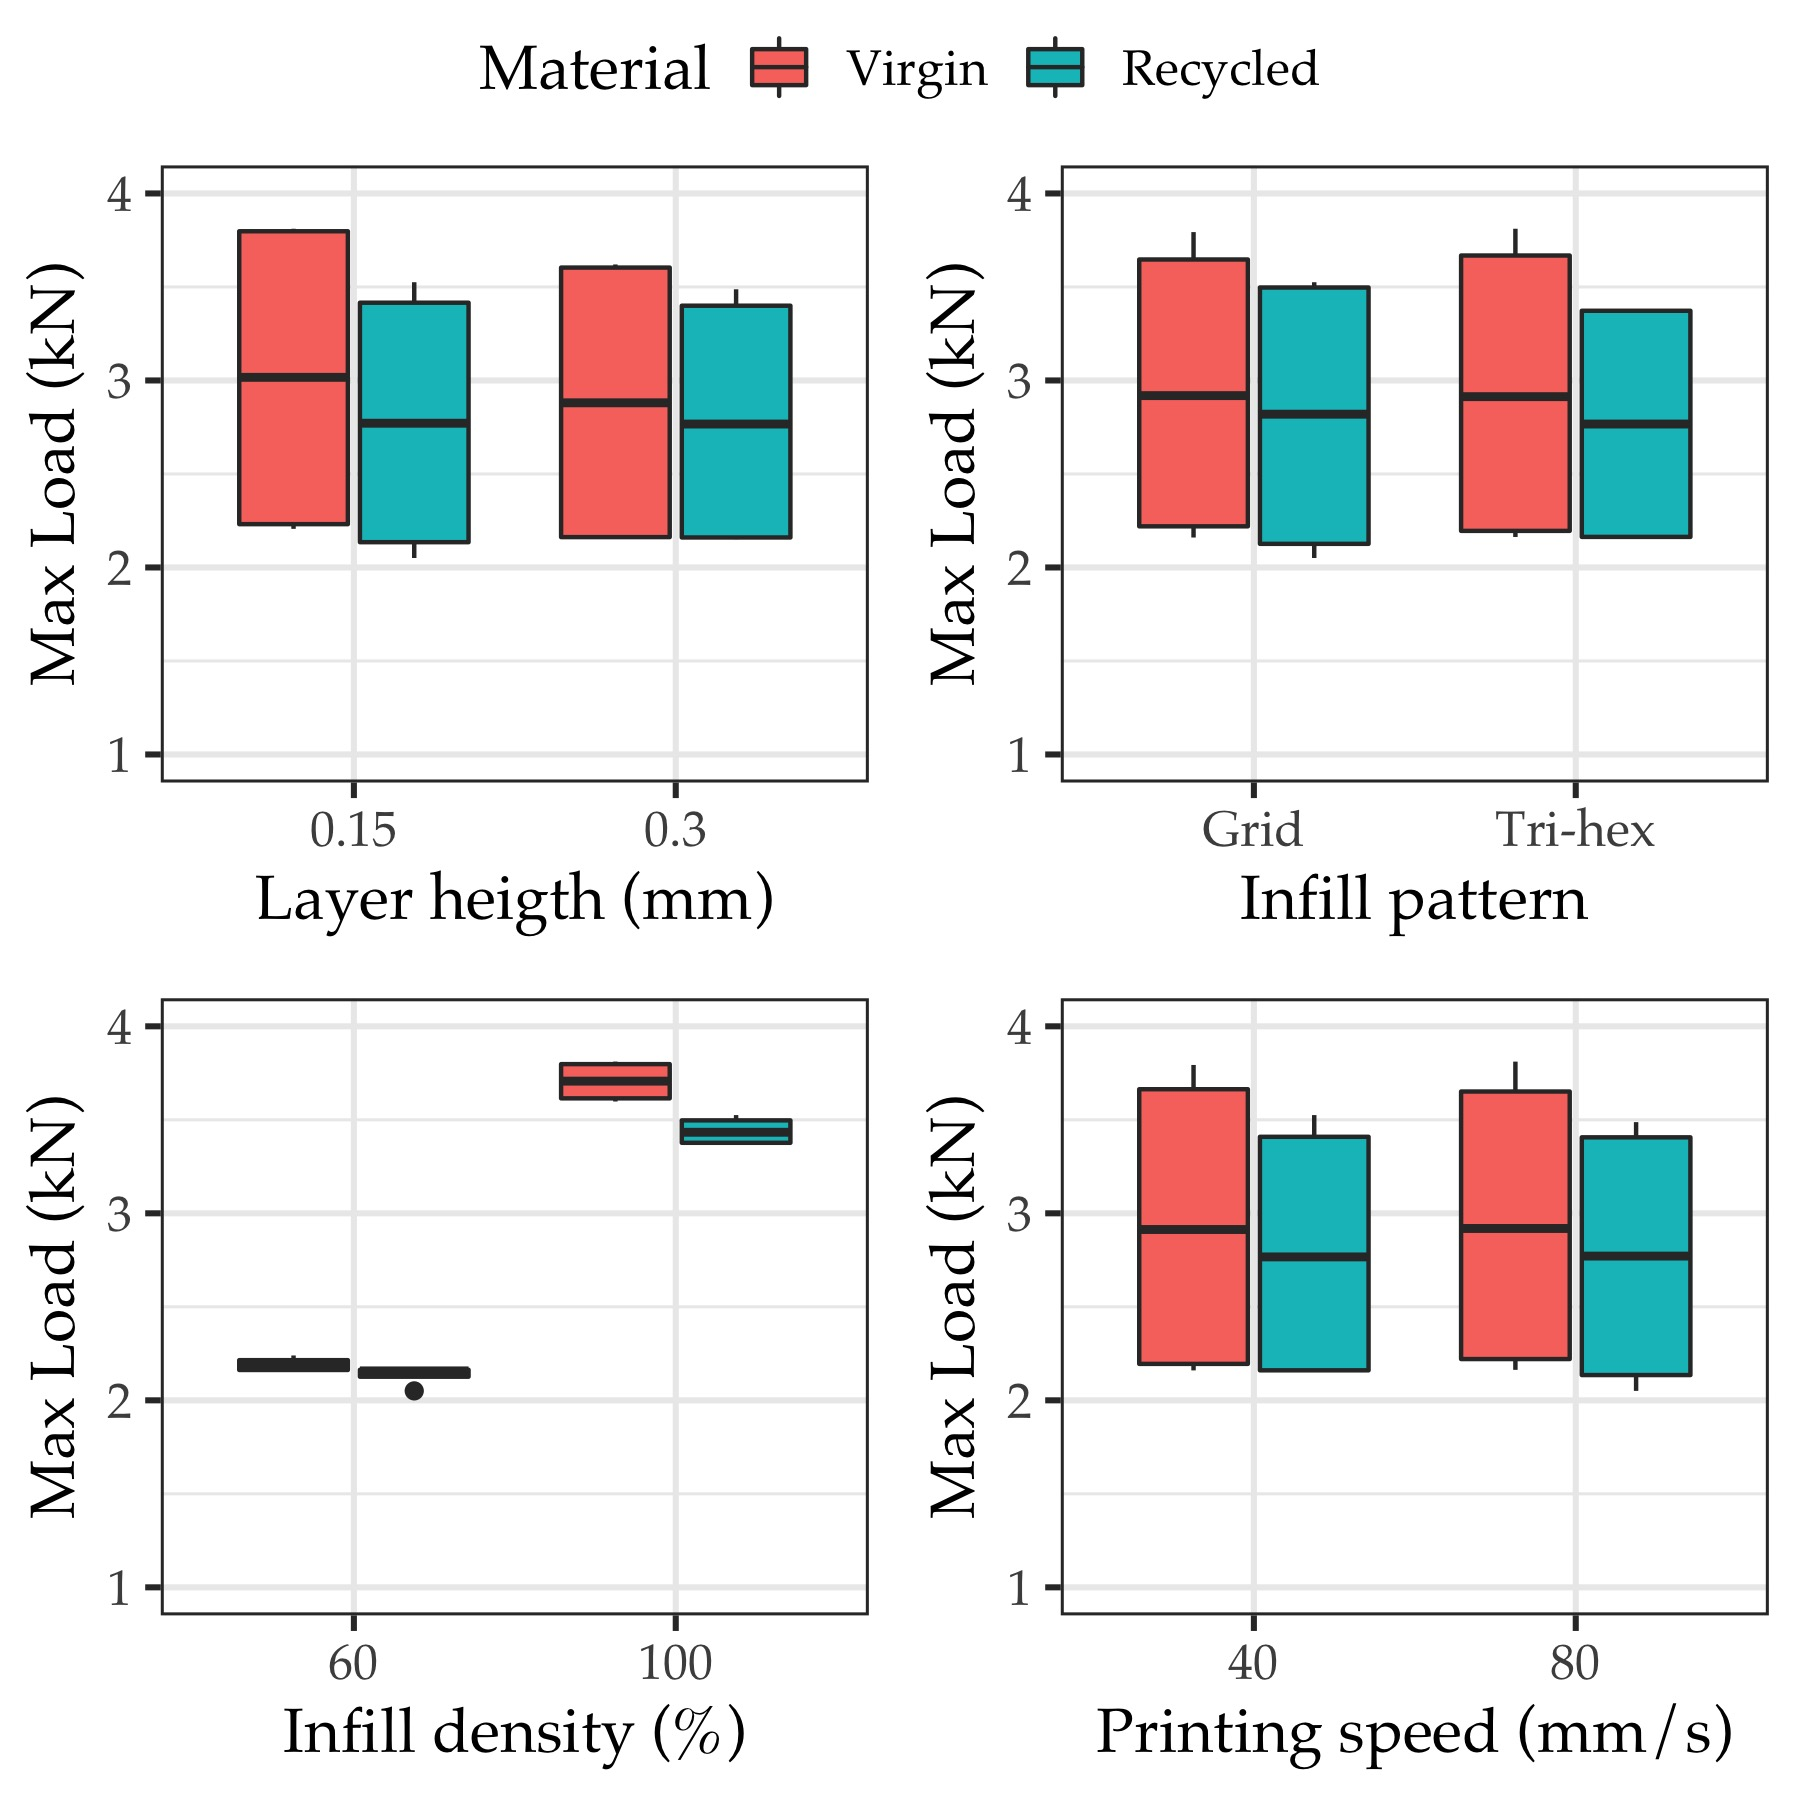
\includegraphics[width=0.40\linewidth]{Figures/Phase-1-2.jpg}%
\label{fig_second_case}}
\caption{Phase 1: screening tests to identify significant factors based on DoE}
\label{Fig:Phase.1b}
\end{figure*}

In general, shortly after attaining the maximum load, the fracture of
the specimen occurred. However, the nature of the fracture was not
homogeneous as shown in Fig \ref{Fig:Phase.1a}. Thus, in most cases, the
specimens showed a fragile behavior and the fracture, either
horizontally or with a lower inclination angle, was clean. However, for
the recycled material, the specimens presented a ductile behavior and,
properly, the fracture did not occur after the maximum load was
attained, canceling the tests minutes after the maximum load was
attained. The breakage in these cases occurred at a 45º angle and, in
the cases of the RE-2 specimen, two parallel fracture lines can be
clearly seen. The printing conditions did not allow us to observe a
clear relation to the fracture of the specimens. This behavior may
relate to that explained by \protect\hyperlink{ref-Yao2019}{{[}19{]}}.
The authors identified two different types of fracture: in-layer and
interlayer. In general, the fracture occurs at the interface of two
layers when printing in vertical position, even when varying the
printing orientation up to 45º from the vertical position. In-layer
fracture is more likely when the specimen is printed using an edgewise
position (or, inclined up to 45º from that position). In this second
case, the printing direction is the same as the tensile stress
direction, which also happens when the horizontal orientation is used.
In these cases, the material layer is not intact after the fracture. As
a result, it is likely that both modes (in-layer and inter-layer
fractures) coexist in this study, which may explain the heterogeneity of
the different fractures.

An analysis of variance (ANOVA) was performed using R software in order
to identify the influential factors on the response variable. As
criterion, critical factors for the response variable were those with
p-values lower than 0.05 \protect\hyperlink{ref-Perez2018}{{[}44{]}}.
Shapiro-Wilk normality tests allowed verifying the normality of the
residuals. The figure \ref{fig:phase-1} illustrates the boxplots of the
results considering each factors. Also, The Table \ref{tab:anova.phase1}
lists the results of the ANOVAs carried out for the experimental
results.

\begin{table}

\caption{\label{tab:Table.Anova.fase1}ANOVA results at 95\% significance level}
\centering
\resizebox{\linewidth}{!}{
\begin{tabular}[t]{lrrrrr}
\toprule
  & Df & Sum Sq & Mean Sq & F value & Pr(F)\\
\midrule
\cellcolor{gray!6}{LH} & \cellcolor{gray!6}{1} & \cellcolor{gray!6}{0.0} & \cellcolor{gray!6}{0.013} & \cellcolor{gray!6}{1.340} & \cellcolor{gray!6}{0.274}\\
IP & 1 & 0.0 & 0.001 & 0.107 & 0.750\\
\cellcolor{gray!6}{ID} & \cellcolor{gray!6}{1} & \cellcolor{gray!6}{8.0} & \cellcolor{gray!6}{7.963} & \cellcolor{gray!6}{824.810} & \cellcolor{gray!6}{0.000}\\
PS & 1 & 0.0 & 0.001 & 0.062 & 0.808\\
\cellcolor{gray!6}{Material} & \cellcolor{gray!6}{1} & \cellcolor{gray!6}{0.1} & \cellcolor{gray!6}{0.106} & \cellcolor{gray!6}{10.957} & \cellcolor{gray!6}{0.008}\\
Residuals & 10 & 0.1 & 0.010 &  & \\
\bottomrule
\end{tabular}}
\end{table}

From the results of the table \ref{tab:anova.phase1} and figure
\ref{fig:phase-1}, it can be clearly identified how the infill density
was the most statistically significant factor for the maximum load
(p-valor lower than 0.001). Likewise, the type of material is also a
significant factor for the response variable but in a less proportion,
being non-significant the rest of the factors. When evaluating the
contribution of each of the factors to the variability explained by the
model, there were calculated values of 97.3 \% and 1.3 \% for infill
density and type of material, respectively. Thus, when manufacturing new
parts or specimens, infill density is a key factor for guaranteeing
adequate mechanical properties of the specimens.

\hypertarget{phase-ii-focusing}{%
\subsection{Phase II: Focusing}\label{phase-ii-focusing}}

The main goal of phase II is the evaluation of the infill density by the
fact that it was observed as a significant factor in the previous phase.
Therefore, five levels of the infill density were chosen ranging from 40
to 100 \% to evaluate the evolution of the maximum load for both virgin
and recycled PLA. The specific levels selected were 40, 55, 70, 85 and
100 \%. Regarding the selection of the other factors of the printing
process, the main criteria was the reduction of time printing as stated
in the methodology section. Therefore, the experimental conditions were
layer height of 0.3 mm, infill pattern tri-hexagonal and printing speed
of 80 mm/s with an estimated printing time of 20 min. A total of 10
samples were manufactured.

\begin{figure}

{\centering 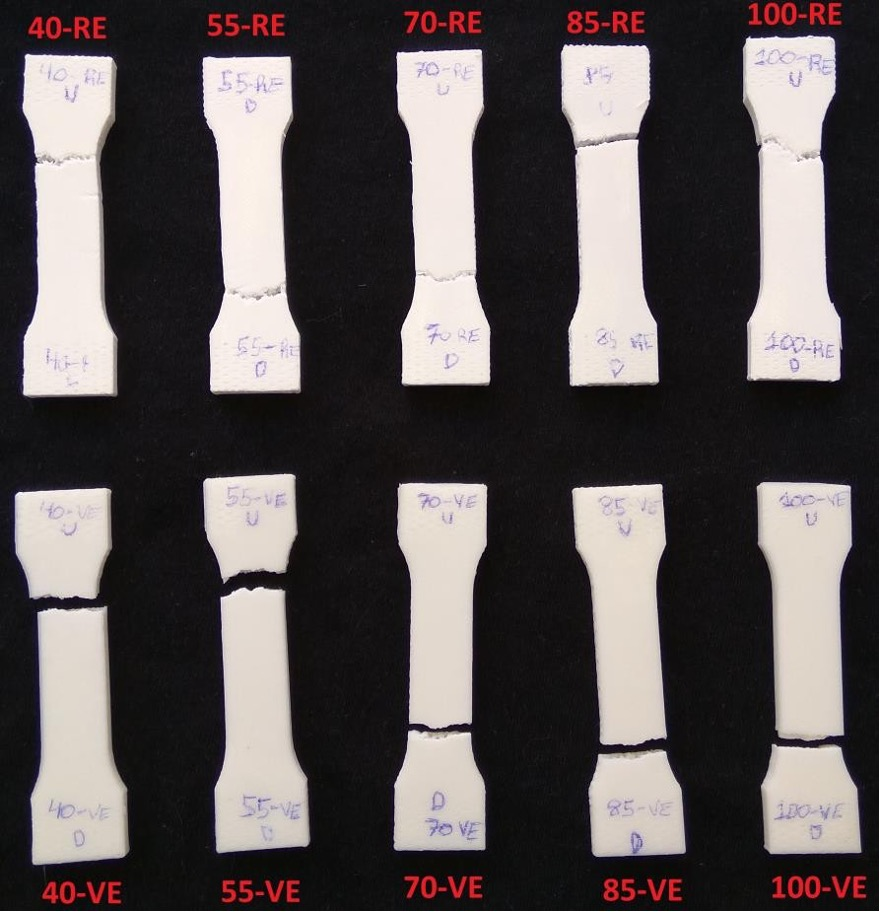
\includegraphics[width=0.8\linewidth]{Figures/Probetas-Fase-2} 

}

\caption{Specimens after tensile test in  phase II. \label{fig:probetas.phase1}}\label{fig:Fig.Probetas.Fase.2}
\end{figure}

Figure \ref{fig:probetas.phase1} shows the fracture of the specimens
tested in phase II. Regarding the fracture, the results were similar as
those of the phase I (i.e., more ductile behavior for the recycled PLA
specimens). The interest element in this phase is presented in Figure
\ref{fig:phase2} where the maximum load versus infill density for both
virgin and recycled PLA are illustrated.

\begin{figure}

{\centering 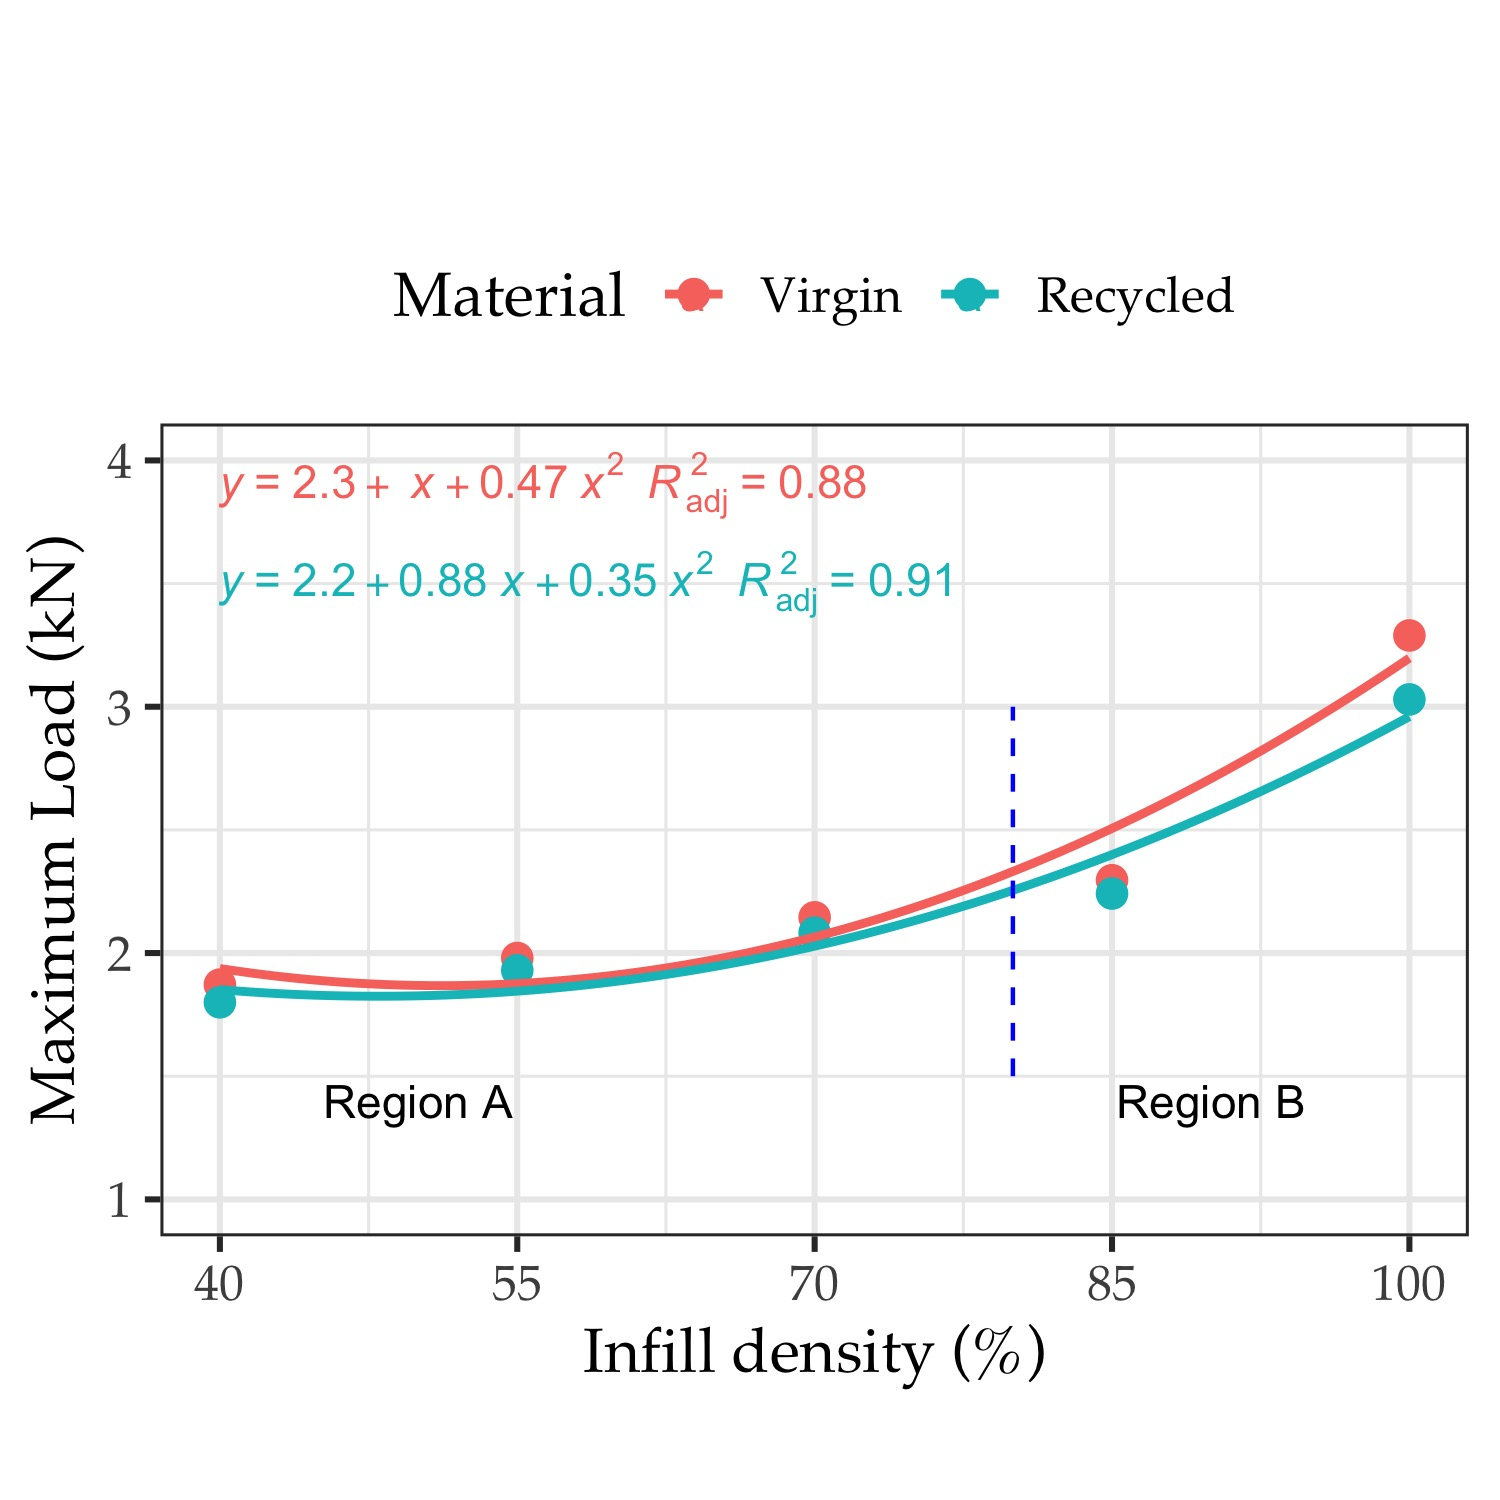
\includegraphics[width=\linewidth]{Figures/Phase-2} 

}

\caption{Maximum load versus infill density for both virgin and recycled PLA. \label{fig:phase2}}\label{fig:Fig.Phase.2}
\end{figure}

From the analysis of the Figure \ref{fig:phase2}, it is possible to
appreciate that there are two clearly different regions. Therefore, in
the A region, comprised between infill densities from 40 to 85 \%, the
slope of the curve grows slowly with a linear trend. Thus, an increase
of the infill density did not provide an proportional increase in the
mechanical properties. due to the fact that the maximum load remained
almost constant. However, in the B region, the slope of the curve grows
largely. Consequently, with a small increase of infill density, the
maximum load notably grows. Regarding the type of material, it is clear
that virgin PLA outperforms recycled PLA, but a reduced difference
between them. These results are in agreement with studies on the
comparison of the performance of recycled and virgin PLA
\protect\hyperlink{ref-CruzSanchez2017}{{[}30{]}} where there was found
a difference of about 10\% of the mechanical properties in the first
recycling cycles. However, the difference notably increased as the
infill density approached 100 \%. The obtained results agree well with
those presented by Wang et al.
\protect\hyperlink{ref-Wang2020h}{{[}45{]}}. In their study, the authors
studied infill density of 20, 40, 60, 80 and 100\% and the evolution of
the tensile strength is similar to the one shown in Figure
\ref{fig:phase2}.

Based on the results, it appears that a reduction from 100\% to 40\% of
infill density implies a relatively reduction in 41.7\% of the maximal
load supported for both type of materials. This is an interesting result
that enables to creation of prototypes with less materials, without
compromising the mechanical solidity. Although the number of measured
points is reduced, it is possible to model the relation between the
maximum load (y) versus the infill density (x) for the two regions and
tested materials by means of polynomial regression that are plotted in
the figure. The models may help to anticipate the mechanical resistance
of a part based on the selection of the infill density. Based on the
developed models, it is possible to highlight that recycled PLA is a
suitable substitute for virgin PLA guaranteeing similar mechanical
resistance. Moreover, by developing models for the mechanical
properties, it is possible to minimize the material consumption for both
virgin and recycled materials satisfying the mechanical resistance
requirements. Thus, by accurately knowing the influence of the printing
conditions on the mechanical resistance, it is possible to advance
towards sustainable manufacturing.

\hypertarget{phase-iii-study-on-the-printing-orientation}{%
\subsection{Phase III: Study on the printing
orientation}\label{phase-iii-study-on-the-printing-orientation}}

In this final phase, the main goal is to test the influence of building
orientation according the established standards by the UNE 116005:2012
(UNE, 2012). Five specimens for each of the orientations (edgewise,
horizontal and vertical ) for both virgin and recycled PLA were
manufactured. The selected printing conditions were infill density of
50\%, printing speed of 80 mm/s, tri-hexagonal infill pattern and layer
height of 0.3 mm, with the objective of limiting the use of material and
the time required for printing.

\begin{figure}

{\centering 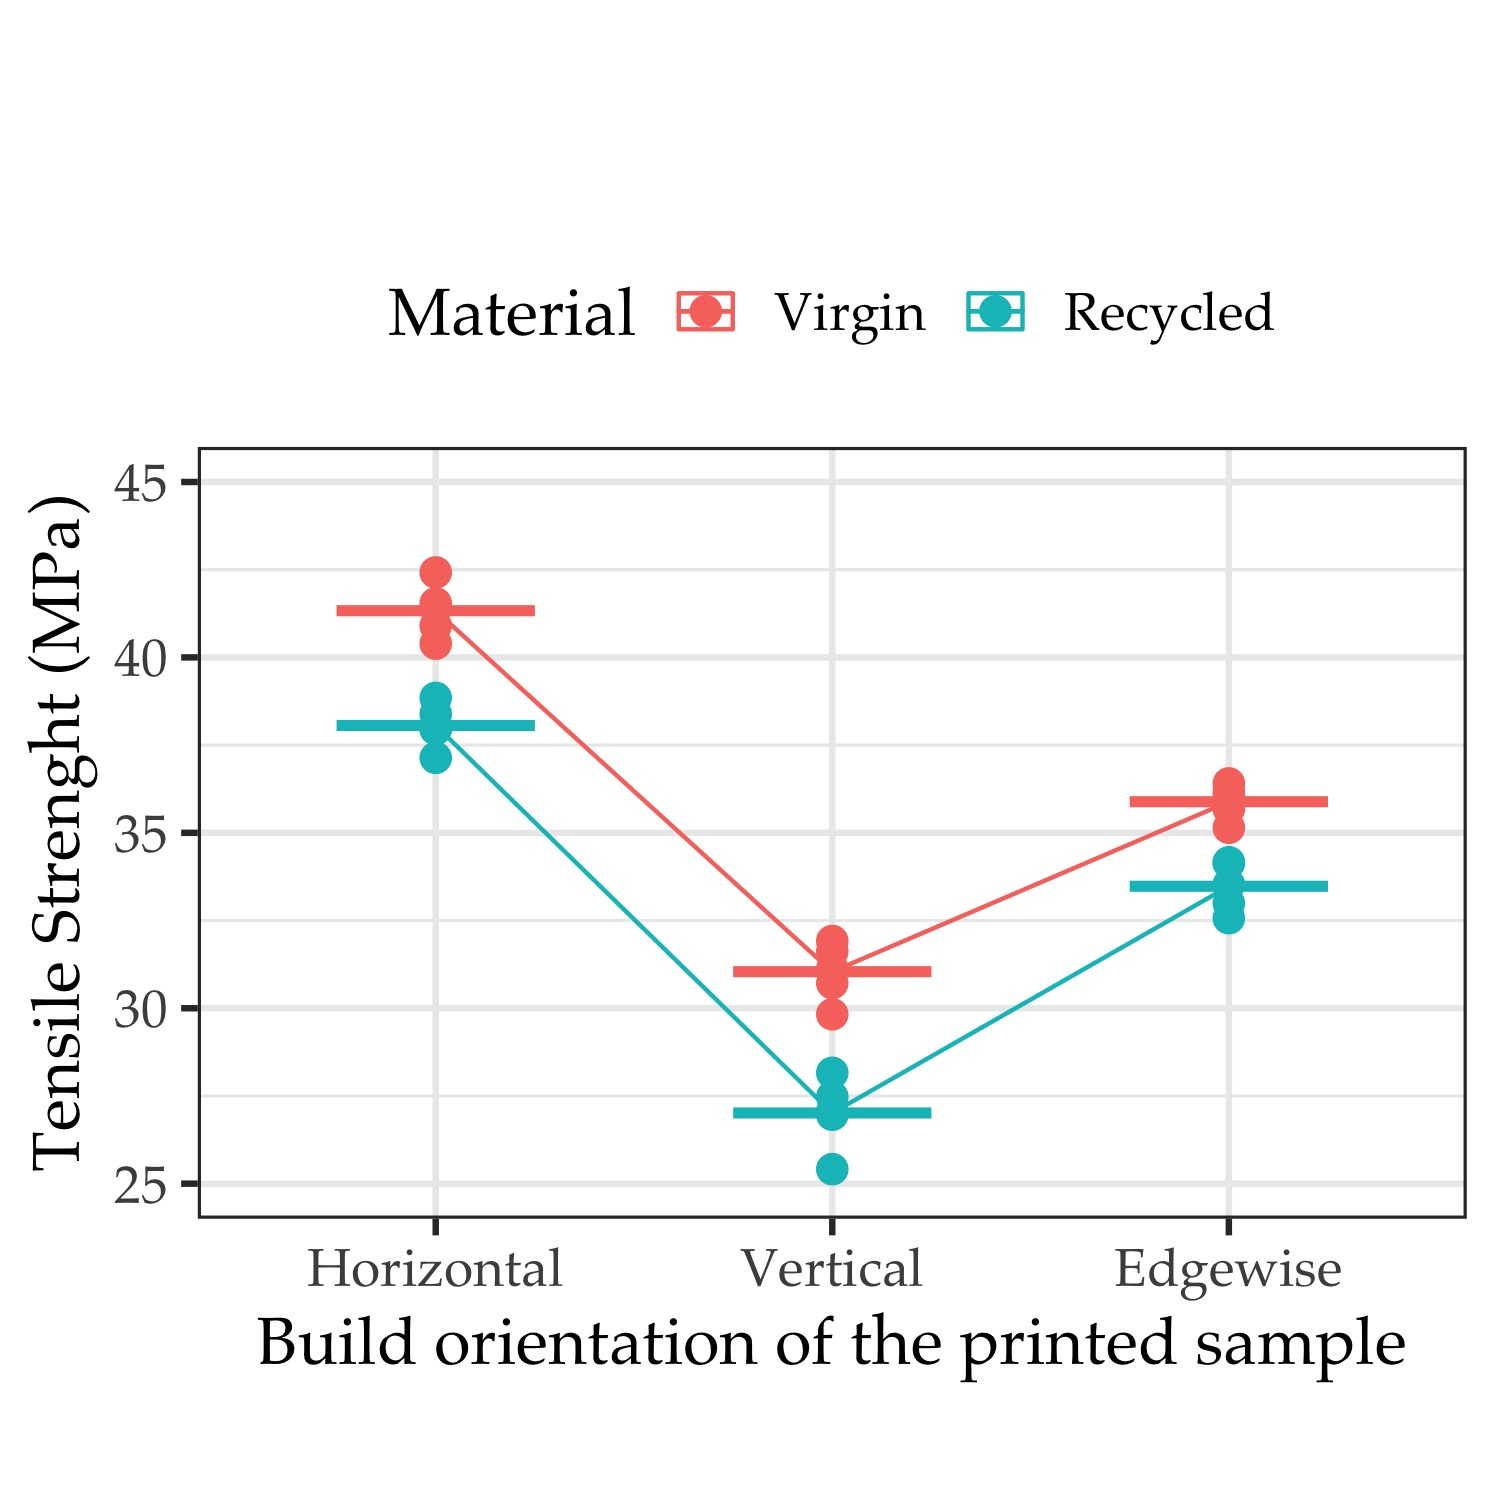
\includegraphics[width=\linewidth]{Figures/Phase-3} 

}

\caption{Average of the load obtain for each build orientation. \label{fig:phase3}}\label{fig:Fig.Phase.3}
\end{figure}

Fig S3 and S4 show the images of the tested specimens observing the same
type of fracture as in the first two phases. It is interesting to
evaluate the reduction in the maximum load depending on the type of
material and orientation in which the specimens were printed.

The Figure \ref{fig:phase3} details the maximum load and the means
values for the five specimens at each orientation. From the results, it
is clear that the horizontal orientation is the one that provided the
higher mechanical resistance, followed by the edgewise orientation.
Likewise, the virgin samples performed better than the recycled samples.

The vertical orientation provided the worse results due to the
deposition of the layers perpendicular to the tensile direction. These
results are in good agreement with those by
\protect\hyperlink{ref-Corapi2019}{{[}46{]}} and
\protect\hyperlink{ref-Wang2020h}{{[}45{]}}. For the recycled material,
there is a slight decrease in the maximum load obtained from 6.71 to
13\% depending on the orientation with respect to the virgin values.
Particularly, the biggest reduction of the load happens in the vertical
orientation with the 13 \%. However, the other two orientations are more
adequate for substituting the virgin material for the recycled material
with a limited reduction in mechanical resistance (6.71 to 7.93 \%).

\hypertarget{discussion-and-limits-of-the-results}{%
\section{Discussion and limits of the
results}\label{discussion-and-limits-of-the-results}}

One of the systemic problems of plastic waste relies on dependency of
the indiscriminate disposal of plastics which carries multiple risks
because many plastic products contain additives that modify their
physico-mechanical properties making it difficult the recycling/reuse
\protect\hyperlink{ref-Wagner2020}{{[}47{]}}. The use of 3D printing
technology for prototyping activities are not excepted of this societal
issue. The main purpose of this article is to see to what extent the
influence of printing parameters affects the tensile resistance of the
printed parts. While a large literature is focused on optimization of
the parameters for obtain functional printed objects using the 100\% of
the printed material, the approach opted here is to observe the
influence of this factor of a large range factors considered as critical
in the using a range. This type approach is important because it enables
designers and users to use printing setups that are envisioned as
prototypes objects, to be secure about the quality of printed products
regarding not using.

One of the main results in this study relies on that infill density of
60\% retains a 58.2\% of the mechanical resistance. This is a relevant
insight for prescriptions of minimal conditions where a printed part can
be manufactured. Moreover, the use of recycled assets in the printing
process, may be a relevant path, considering the current priorities of
EU on circular economy and carbon neutral strategies ambitions. Also,
there is a great development of applications using distributed recycling
approach. For instance, Nur-A-Tomal et al
\protect\hyperlink{ref-Nur-A-Tomal2020}{{[}48{]}} presented a valuable
example of waste-to-wealth to use waste plastic toys retaining the
original colour of waste plastic to fabricate new products. Certainly,
the development of complete closed loop DRAM case studies based on
material and location to demonstrate technical, ecological and economic
feasibility \protect\hyperlink{ref-CruzSanchez2020}{{[}25{]}}.

There are certain limitations to this work in the perspective of
materials and parameters tested. Certainly, the use of other materials
is needed to evaluate if the influence of infill and recycled material
are consequent with the results found. Moreover, other major factors are
needed in order to consider the quality of a prototype. Clearly, in the
prototypes where the main goal is the user acceptability, surface/text
finishing, dimensional accuracy are key variables to include for the
printed objects rather than mechanical resistance. Nevertheless, this is
an ongoing research in which the main purpose is to promote the use. The
validation statistical validation of the influence of minimal
parameters.

\hypertarget{conclusions}{%
\section{Conclusions}\label{conclusions}}

The present study includes a comprehensive experimental program to
analyze the Fused Filament Fabrication process based on mechanical
resistance using virgin PLA and recycled PLA. The paper aims at
improving the sustainability of 3D printing process, assessing the
technical feasibility of the substitution. The main conclusions of the
study are the following. The printing conditions determined in a great
manner the mechanical resistance of the specimens. Specifically, the
most influential factor on the maximum load for both virgin and recycled
PLA was the infill density.\\
The influence of the infill density on the maximum load allowed
identifying two different regions: A, from 40 to 85 \%, linear behavior
with a slight slope and, B, from 85 to 100 \%, the maximum load
increases notably with a much higher slope. The fracture for the virgin
material corresponded to that of a fragile material, while the fracture
of the recycled material showed a more ductile behavior.

The selected orientation for printing the specimens is of great
importance for the maximum load because of the anisotropy. In this
sense, the horizontal orientation allowed attaining a higher maximum
load, while the vertical orientation provided the lower value due to the
fact that no layers were deposited in the tensile direction. Our results
support the main argument on the substitution of virgin PLA for recycled
PLA based on the mechanical resistance for prototyping purposes,
advancing towards sustainable manufacturing. Is was found that using an
infill density of 40\%, there is a retention of the 58.2\% of the
mechanical resistance. Despite recycled PLA offers a slightly lower
mechanical resistance, when possible, by properly selecting the printing
conditions (mainly, by the infill density and orientation) it could be
approximate to that of the virgin PLA. Particularly, when using edgewise
and horizontal orientations it is possible to obtain maximum loads close
to that of the virgin material (from 3 to 8 \% lower).

\hypertarget{acknowledgments}{%
\section{ACKNOWLEDGMENTS}\label{acknowledgments}}

The authors would like to thank the ``Mechanical and Energy
Engineering'' TEP 250 research group and to the Lorraine Fab Living Lab.
This research is partially funded from the European Union's Horizon 2020
research and innovation programme under grant agreement No 869952.

\hypertarget{references}{%
\section*{References}\label{references}}
\addcontentsline{toc}{section}{References}

\hypertarget{refs}{}
\begin{CSLReferences}{0}{0}
\leavevmode\hypertarget{ref-Jin2017}{}%
\CSLLeftMargin{{[}1{]} }
\CSLRightInline{Y. Jin, Y. Wan, B. Zhang, and Z. Liu, {``{Modeling of
the chemical finishing process for polylactic acid parts in fused
deposition modeling and investigation of its tensile properties},''}
\emph{J. Mater. Process. Technol.}, vol. 240, pp. 233--239, Feb. 2017,
doi:
\href{https://doi.org/10.1016/j.jmatprotec.2016.10.003}{10.1016/j.jmatprotec.2016.10.003}.}

\leavevmode\hypertarget{ref-Xiao2014}{}%
\CSLLeftMargin{{[}2{]} }
\CSLRightInline{K. Xiao, F. Zardawi, R. Van Noort, and J. M. Yates,
{``{Developing a 3D colour image reproduction system for additive
manufacturing of facial prostheses},''} \emph{Int. J. Adv. Manuf.
Technol.}, vol. 70, no. 9--12, pp. 2043--2049, Feb. 2014, doi:
\href{https://doi.org/10.1007/s00170-013-5448-1}{10.1007/s00170-013-5448-1}.}

\leavevmode\hypertarget{ref-Peng2018}{}%
\CSLLeftMargin{{[}3{]} }
\CSLRightInline{T. Peng, K. Kellens, R. Tang, C. Chen, and G. Chen,
{``{Sustainability of additive manufacturing: An overview on its energy
demand and environmental impact},''} \emph{Addit. Manuf.}, vol. 21, no.
June 2017, pp. 694--704, May 2018, doi:
\href{https://doi.org/10.1016/j.addma.2018.04.022}{10.1016/j.addma.2018.04.022}.}

\leavevmode\hypertarget{ref-Niaki2019}{}%
\CSLLeftMargin{{[}4{]} }
\CSLRightInline{M. K. Niaki, S. A. Torabi, and F. Nonino, {``{Why
manufacturers adopt additive manufacturing technologies: The role of
sustainability},''} \emph{J. Clean. Prod.}, vol. 222, pp. 381--392, Jun.
2019, doi:
\href{https://doi.org/10.1016/j.jclepro.2019.03.019}{10.1016/j.jclepro.2019.03.019}.}

\leavevmode\hypertarget{ref-Despeisse2016}{}%
\CSLLeftMargin{{[}5{]} }
\CSLRightInline{M. Despeisse \emph{et al.}, {``{Unlocking value for a
circular economy through 3D printing: A research agenda},''}
\emph{Technol. Forecast. Soc. Change}, vol. 115, pp. 75--84, Feb. 2017,
doi:
\href{https://doi.org/10.1016/j.techfore.2016.09.021}{10.1016/j.techfore.2016.09.021}.}

\leavevmode\hypertarget{ref-GonzalezHenriquez2019}{}%
\CSLLeftMargin{{[}6{]} }
\CSLRightInline{C. M. González-Henríquez, M. A. Sarabia-Vallejos, and J.
Rodriguez-Hernandez, {``{Polymers for additive manufacturing and
4D-printing: Materials, methodologies, and biomedical applications},''}
\emph{Prog. Polym. Sci.}, vol. 94, pp. 57--116, Jul. 2019, doi:
\href{https://doi.org/10.1016/j.progpolymsci.2019.03.001}{10.1016/j.progpolymsci.2019.03.001}.}

\leavevmode\hypertarget{ref-Ryberg2019}{}%
\CSLLeftMargin{{[}7{]} }
\CSLRightInline{M. W. Ryberg, M. Z. Hauschild, F. Wang, S.
Averous-Monnery, and A. Laurent, {``{Global environmental losses of
plastics across their value chains},''} \emph{Resour. Conserv. Recycl.},
vol. 151, p. 104459, Dec. 2019, doi:
\href{https://doi.org/10.1016/j.resconrec.2019.104459}{10.1016/j.resconrec.2019.104459}.}

\leavevmode\hypertarget{ref-Elverum2016a}{}%
\CSLLeftMargin{{[}8{]} }
\CSLRightInline{C. W. Elverum, T. Welo, and S. Tronvoll, {``{Prototyping
in New Product Development: Strategy Considerations},''} in
\emph{Procedia CIRP}, 2016, vol. 50, pp. 117--122, doi:
\href{https://doi.org/10.1016/j.procir.2016.05.010}{10.1016/j.procir.2016.05.010}.}

\leavevmode\hypertarget{ref-Menold2017}{}%
\CSLLeftMargin{{[}9{]} }
\CSLRightInline{J. Menold, K. Jablokow, and T. Simpson, {``{Prototype
for X (PFX): A holistic framework for structuring prototyping methods to
support engineering design},''} \emph{Des. Stud.}, vol. 50, pp. 70--112,
2017, doi:
\href{https://doi.org/10.1016/j.destud.2017.03.001}{10.1016/j.destud.2017.03.001}.}

\leavevmode\hypertarget{ref-Elverum2016}{}%
\CSLLeftMargin{{[}10{]} }
\CSLRightInline{C. W. Elverum, T. Welo, and S. Tronvoll, {``{Prototyping
in New Product Development: Strategy Considerations},''} in
\emph{Procedia CIRP}, 2016, vol. 50, pp. 117--122, doi:
\href{https://doi.org/10.1016/j.procir.2016.05.010}{10.1016/j.procir.2016.05.010}.}

\leavevmode\hypertarget{ref-Wolszczak2018}{}%
\CSLLeftMargin{{[}11{]} }
\CSLRightInline{P. Wolszczak, K. Lygas, M. Paszko, and R. A. Wach,
{``{Heat distribution in material during fused deposition modelling},''}
\emph{Rapid Prototyp. J.}, vol. 24, no. 3, pp. 615--622, Apr. 2018, doi:
\href{https://doi.org/10.1108/RPJ-04-2017-0062}{10.1108/RPJ-04-2017-0062}.}

\leavevmode\hypertarget{ref-Chua2017}{}%
\CSLLeftMargin{{[}12{]} }
\CSLRightInline{C. K. Chua, C. H. Wong, and W. Y. Yeong, {``{Standards,
quality control, and measurement sciences in 3D printing and additive
manufacturing}.''} Academic Press, 2017.}

\leavevmode\hypertarget{ref-Zhao2018a}{}%
\CSLLeftMargin{{[}13{]} }
\CSLRightInline{X. G. Zhao, K.-J. Hwang, D. Lee, T. Kim, and N. Kim,
{``{Enhanced mechanical properties of self-polymerized
polydopamine-coated recycled PLA filament used in 3D printing},''}
\emph{Appl. Surf. Sci.}, vol. 441, pp. 381--387, May 2018, doi:
\href{https://doi.org/10.1016/j.apsusc.2018.01.257}{10.1016/j.apsusc.2018.01.257}.}

\leavevmode\hypertarget{ref-Singh2018e}{}%
\CSLLeftMargin{{[}14{]} }
\CSLRightInline{R. Singh, R. Kumar, and P. Singh, {``{Prospect of 3D
Printing for Recycling of Plastic Product to Minimize Environmental
Pollution},''} in \emph{Ref. Modul. Mater. Sci. Mater. eng.}, Elsevier,
2018, pp. 1--14.}

\leavevmode\hypertarget{ref-Laureto2018}{}%
\CSLLeftMargin{{[}15{]} }
\CSLRightInline{J. J. Laureto and J. M. Pearce, {``{Anisotropic
mechanical property variance between ASTM D638-14 type i and type iv
fused filament fabricated specimens},''} \emph{Polym. Test.}, vol. 68,
no. March, pp. 294--301, 2018, doi:
\href{https://doi.org/10.1016/j.polymertesting.2018.04.029}{10.1016/j.polymertesting.2018.04.029}.}

\leavevmode\hypertarget{ref-Popescu2018}{}%
\CSLLeftMargin{{[}16{]} }
\CSLRightInline{D. Popescu, A. Zapciu, C. Amza, F. Baciu, and R.
Marinescu, {``{FDM process parameters influence over the mechanical
properties of polymer specimens: A review},''} \emph{Polym. Test.}, vol.
69, pp. 157--166, 2018, doi:
\href{https://doi.org/10.1016/j.polymertesting.2018.05.020}{10.1016/j.polymertesting.2018.05.020}.}

\leavevmode\hypertarget{ref-CruzSanchez2014}{}%
\CSLLeftMargin{{[}17{]} }
\CSLRightInline{F. A. Cruz Sanchez, H. Boudaoud, L. Muller, and M.
Camargo, {``{Towards a standard experimental protocol for open source
additive manufacturing},''} \emph{Virtual Phys. Prototyp.}, vol. 9, no.
3, pp. 151--167, Jul. 2014, doi:
\href{https://doi.org/10.1080/17452759.2014.919553}{10.1080/17452759.2014.919553}.}

\leavevmode\hypertarget{ref-JaisinghSheoran2019}{}%
\CSLLeftMargin{{[}18{]} }
\CSLRightInline{A. Jaisingh Sheoran and H. Kumar, {``{Fused Deposition
modeling process parameters optimization and effect on mechanical
properties and part quality: Review and reflection on present
research},''} in \emph{Mater. Today proc.}, 2020, vol. 21, pp.
1659--1672, doi:
\href{https://doi.org/10.1016/j.matpr.2019.11.296}{10.1016/j.matpr.2019.11.296}.}

\leavevmode\hypertarget{ref-Yao2019}{}%
\CSLLeftMargin{{[}19{]} }
\CSLRightInline{T. Yao, Z. Deng, K. Zhang, and S. Li, {``{A method to
predict the ultimate tensile strength of 3D printing polylactic acid
(PLA) materials with different printing orientations},''} \emph{Compos.
Part B Eng.}, vol. 163, pp. 393--402, 2019, doi:
\href{https://doi.org/10.1016/j.compositesb.2019.01.025}{10.1016/j.compositesb.2019.01.025}.}

\leavevmode\hypertarget{ref-Alafaghani2018}{}%
\CSLLeftMargin{{[}20{]} }
\CSLRightInline{A. aldin Alafaghani and A. Qattawi, {``{Investigating
the effect of fused deposition modeling processing parameters using
Taguchi design of experiment method},''} \emph{J. Manuf. Process.}, vol.
36, pp. 164--174, Dec. 2018, doi:
\href{https://doi.org/10.1016/j.jmapro.2018.09.025}{10.1016/j.jmapro.2018.09.025}.}

\leavevmode\hypertarget{ref-Altan2018}{}%
\CSLLeftMargin{{[}21{]} }
\CSLRightInline{M. Altan, M. Eryildiz, B. Gumus, and Y. Kahraman,
{``{Effects of process parameters on the quality of PLA products
fabricated by fused deposition modeling (FDM): Surface roughness and
tensile strength},''} \emph{Mater. Test.}, vol. 60, no. 5, pp. 471--477,
May 2018, doi:
\href{https://doi.org/10.3139/120.111178}{10.3139/120.111178}.}

\leavevmode\hypertarget{ref-Ashby2013}{}%
\CSLLeftMargin{{[}22{]} }
\CSLRightInline{M. F. Ashby and K. Johnson, \emph{{Materials and design:
the art and science of material selection in product design}}.
Butterworth-Heinemann, 2013.}

\leavevmode\hypertarget{ref-Liu2019a}{}%
\CSLLeftMargin{{[}23{]} }
\CSLRightInline{J. Liu, L. Sun, W. Xu, Q. Wang, S. Yu, and J. Sun,
{``{Current advances and future perspectives of 3D printing
natural-derived biopolymers},''} \emph{Carbohydr. Polym.}, vol. 207, pp.
297--316, Mar. 2019, doi:
\href{https://doi.org/10.1016/j.carbpol.2018.11.077}{10.1016/j.carbpol.2018.11.077}.}

\leavevmode\hypertarget{ref-Kumar2018b}{}%
\CSLLeftMargin{{[}24{]} }
\CSLRightInline{R. Kumar, R. Singh, and I. Farina, {``{On the 3D
printing of recycled ABS, PLA and HIPS thermoplastics for structural
applications},''} \emph{PSU Res. Rev.}, vol. 2, no. 2, pp. 115--137,
Aug. 2018, doi:
\href{https://doi.org/10.1108/prr-07-2018-0018}{10.1108/prr-07-2018-0018}.}

\leavevmode\hypertarget{ref-CruzSanchez2020}{}%
\CSLLeftMargin{{[}25{]} }
\CSLRightInline{F. A. Cruz Sanchez, H. Boudaoud, M. Camargo, and J. M.
Pearce, {``{Plastic recycling in additive manufacturing: A systematic
literature review and opportunities for the circular economy},''}
\emph{J. Clean. Prod.}, vol. 264, p. 121602, Aug. 2020, doi:
\href{https://doi.org/10.1016/j.jclepro.2020.121602}{10.1016/j.jclepro.2020.121602}.}

\leavevmode\hypertarget{ref-Little2020}{}%
\CSLLeftMargin{{[}26{]} }
\CSLRightInline{H. A. Little, N. G. Tanikella, M. J. Reich, M. J.
Fiedler, S. L. Snabes, and J. M. Pearce, {``{Towards Distributed
Recycling with Additive Manufacturing of PET Flake Feedstocks},''}
\emph{Materials (Basel).}, vol. 13, no. 19, p. 4273, Sep. 2020, doi:
\href{https://doi.org/10.3390/ma13194273}{10.3390/ma13194273}.}

\leavevmode\hypertarget{ref-Zhao2018}{}%
\CSLLeftMargin{{[}27{]} }
\CSLRightInline{P. Zhao, C. Rao, F. Gu, N. Sharmin, and J. Fu,
{``{Close-looped recycling of polylactic acid used in 3D printing: An
experimental investigation and life cycle assessment},''} \emph{J.
Clean. Prod.}, vol. 197, pp. 1046--1055, Oct. 2018, doi:
\href{https://doi.org/10.1016/j.jclepro.2018.06.275}{10.1016/j.jclepro.2018.06.275}.}

\leavevmode\hypertarget{ref-Petrovic2011}{}%
\CSLLeftMargin{{[}28{]} }
\CSLRightInline{V. Petrovic, J. Vicente Haro Gonzalez, O. Jordá
Ferrando, J. Delgado Gordillo, J. Ramón Blasco Puchades, and L. Portolés
Griñan, {``{Additive layered manufacturing: sectors of industrial
application shown through case studies},''} \emph{Int. J. Prod. Res.},
vol. 49, no. 4, pp. 1061--1079, Feb. 2011, doi:
\href{https://doi.org/10.1080/00207540903479786}{10.1080/00207540903479786}.}

\leavevmode\hypertarget{ref-Santander2020}{}%
\CSLLeftMargin{{[}29{]} }
\CSLRightInline{P. Santander, F. A. Cruz Sanchez, H. Boudaoud, and M.
Camargo, {``{Closed loop supply chain network for local and distributed
plastic recycling for 3D printing: a MILP-based optimization
approach},''} \emph{Resour. Conserv. Recycl.}, vol. 154, p. 104531, Mar.
2020, doi:
\href{https://doi.org/10.1016/j.resconrec.2019.104531}{10.1016/j.resconrec.2019.104531}.}

\leavevmode\hypertarget{ref-CruzSanchez2017}{}%
\CSLLeftMargin{{[}30{]} }
\CSLRightInline{F. A. Cruz Sanchez, H. Boudaoud, S. Hoppe, and M.
Camargo, {``{Polymer recycling in an open-source additive manufacturing
context: Mechanical issues},''} \emph{Addit. Manuf.}, vol. 17, pp.
87--105, Oct. 2017, doi:
\href{https://doi.org/10.1016/j.addma.2017.05.013}{10.1016/j.addma.2017.05.013}.}

\leavevmode\hypertarget{ref-Vidakis2020}{}%
\CSLLeftMargin{{[}31{]} }
\CSLRightInline{N. Vidakis, M. Petousis, A. Maniadi, E. Koudoumas, A.
Vairis, and J. Kechagias, {``{Sustainable additive manufacturing:
Mechanical response of acrylonitrile-butadiene-styrene over multiple
recycling processes},''} \emph{Sustain.}, vol. 12, no. 9, 2020, doi:
\href{https://doi.org/10.3390/SU12093568}{10.3390/SU12093568}.}

\leavevmode\hypertarget{ref-Zander2018}{}%
\CSLLeftMargin{{[}32{]} }
\CSLRightInline{N. E. Zander, M. Gillan, and R. H. Lambeth, {``{Recycled
polyethylene terephthalate as a new FFF feedstock material},''}
\emph{Addit. Manuf.}, vol. 21, no. January, pp. 174--182, May 2018, doi:
\href{https://doi.org/10.1016/j.addma.2018.03.007}{10.1016/j.addma.2018.03.007}.}

\leavevmode\hypertarget{ref-Gu2016}{}%
\CSLLeftMargin{{[}33{]} }
\CSLRightInline{F. Gu, P. Hall, and N. J. Miles, {``{Performance
evaluation for composites based on recycled polypropylene using
principal component analysis and cluster analysis},''} \emph{J. Clean.
Prod.}, vol. 115, pp. 343--353, Mar. 2016, doi:
\href{https://doi.org/10.1016/j.jclepro.2015.12.062}{10.1016/j.jclepro.2015.12.062}.}

\leavevmode\hypertarget{ref-Babagowda2018}{}%
\CSLLeftMargin{{[}34{]} }
\CSLRightInline{Babagowda, R. S. Kadadevara Math, R. Goutham, and K. R.
Srinivas Prasad, {``{Study of Effects on Mechanical Properties of PLA
Filament which is blended with Recycled PLA Materials},''} \emph{IOP
Conf. Ser. Mater. Sci. Eng.}, vol. 310, no. 1, p. 012103, Feb. 2018,
doi:
\href{https://doi.org/10.1088/1757-899X/310/1/012103}{10.1088/1757-899X/310/1/012103}.}

\leavevmode\hypertarget{ref-Pinho2020}{}%
\CSLLeftMargin{{[}35{]} }
\CSLRightInline{A. C. Pinho, A. M. Amaro, and A. P. Piedade, {``{3D
printing goes greener: Study of the properties of post-consumer recycled
polymers for the manufacturing of engineering components},''}
\emph{Waste Manag.}, vol. 118, pp. 426--434, 2020, doi:
\href{https://doi.org/10.1016/j.wasman.2020.09.003}{10.1016/j.wasman.2020.09.003}.}

\leavevmode\hypertarget{ref-Suarez2020}{}%
\CSLLeftMargin{{[}36{]} }
\CSLRightInline{L. Suárez and M. Domínguez, {``{Sustainability and
environmental impact of fused deposition modelling (FDM)
technologies},''} \emph{Int. J. Adv. Manuf. Technol.}, vol. 106, no.
3--4, pp. 1267--1279, 2020, doi:
\href{https://doi.org/10.1007/s00170-019-04676-0}{10.1007/s00170-019-04676-0}.}

\leavevmode\hypertarget{ref-Lanzotti2019}{}%
\CSLLeftMargin{{[}37{]} }
\CSLRightInline{A. Lanzotti, M. Martorelli, S. Maietta, S. Gerbino, F.
Penta, and A. Gloria, {``{A comparison between mechanical properties of
specimens 3D printed with virgin and recycled PLA},''} \emph{Procedia
CIRP}, vol. 79, pp. 143--146, 2019, doi:
\href{https://doi.org/10.1016/j.procir.2019.02.030}{10.1016/j.procir.2019.02.030}.}

\leavevmode\hypertarget{ref-Lin2018}{}%
\CSLLeftMargin{{[}38{]} }
\CSLRightInline{W. Lin, H. Shen, G. Xu, L. Zhang, J. Fu, and X. Deng,
{``{Single-layer temperature-adjusting transition method to improve the
bond strength of 3D-printed PCL/PLA parts},''} \emph{Compos. Part A
Appl. Sci. Manuf.}, vol. 115, pp. 22--30, Dec. 2018, doi:
\href{https://doi.org/10.1016/j.compositesa.2018.09.008}{10.1016/j.compositesa.2018.09.008}.}

\leavevmode\hypertarget{ref-Montgomery2001}{}%
\CSLLeftMargin{{[}39{]} }
\CSLRightInline{D. C. Montgomery, \emph{{Design and Analysis of
Experiments}}. 2001.}

\leavevmode\hypertarget{ref-Chacon2017}{}%
\CSLLeftMargin{{[}40{]} }
\CSLRightInline{J. M. Chacón, M. A. Caminero, E. García-Plaza, and P. J.
Núñez, {``{Additive manufacturing of PLA structures using fused
deposition modelling: Effect of process parameters on mechanical
properties and~their optimal selection},''} \emph{Mater. Des.}, vol.
124, pp. 143--157, 2017, doi:
\href{https://doi.org/10.1016/j.matdes.2017.03.065}{10.1016/j.matdes.2017.03.065}.}

\leavevmode\hypertarget{ref-Letcher2015}{}%
\CSLLeftMargin{{[}41{]} }
\CSLRightInline{T. Letcher, B. Rankouhi, and S. Javadpour,
{``{Experimental study of mechanical properties of additively
manufactured abs plastic as a function of layer parameters},''} in
\emph{ASME int. Mech. Eng. Congr. Expo. proc.}, 2015, vol. 2A--2015,
doi:
\href{https://doi.org/10.1115/IMECE2015-52634}{10.1115/IMECE2015-52634}.}

\leavevmode\hypertarget{ref-Singh2019}{}%
\CSLLeftMargin{{[}42{]} }
\CSLRightInline{R. Singh, H. Singh, I. Farina, F. Colangelo, and F.
Fraternali, {``{On the additive manufacturing of an energy storage
device from recycled material},''} \emph{Compos. Part B Eng.}, vol. 156,
pp. 259--265, Jan. 2019, doi:
\href{https://doi.org/10.1016/j.compositesb.2018.08.080}{10.1016/j.compositesb.2018.08.080}.}

\leavevmode\hypertarget{ref-Tanveer2019}{}%
\CSLLeftMargin{{[}43{]} }
\CSLRightInline{Md. Q. Tanveer, A. Haleem, and M. Suhaib, {``{Effect of
variable infill density on mechanical behaviour of 3-D printed PLA
specimen: an experimental investigation},''} \emph{SN Appl. Sci.}, vol.
1, no. 12, pp. 1--12, Dec. 2019, doi:
\href{https://doi.org/10.1007/s42452-019-1744-1}{10.1007/s42452-019-1744-1}.}

\leavevmode\hypertarget{ref-Perez2018}{}%
\CSLLeftMargin{{[}44{]} }
\CSLRightInline{M. Pérez, G. Medina-Sánchez, A. García-Collado, M.
Gupta, and D. Carou, {``{Surface quality enhancement of fused deposition
modeling (FDM) printed samples based on the selection of critical
printing parameters},''} \emph{Materials (Basel).}, vol. 11, no. 8, p.
1382, Aug. 2018, doi:
\href{https://doi.org/10.3390/ma11081382}{10.3390/ma11081382}.}

\leavevmode\hypertarget{ref-Wang2020h}{}%
\CSLLeftMargin{{[}45{]} }
\CSLRightInline{S. Wang, Y. Ma, Z. Deng, S. Zhang, and J. Cai,
{``{Effects of fused deposition modeling process parameters on tensile,
dynamic mechanical properties of 3D printed polylactic acid
materials},''} \emph{Polym. Test.}, vol. 86, 2020, doi:
\href{https://doi.org/10.1016/j.polymertesting.2020.106483}{10.1016/j.polymertesting.2020.106483}.}

\leavevmode\hypertarget{ref-Corapi2019}{}%
\CSLLeftMargin{{[}46{]} }
\CSLRightInline{D. Corapi, G. Morettini, G. Pascoletti, and C. Zitelli,
{``{Characterization of a polylactic acid (PLA) produced by Fused
Deposition Modeling (FDM) technology},''} in \emph{Procedia struct.
integr.}, 2019, vol. 24, pp. 289--295, doi:
\href{https://doi.org/10.1016/j.prostr.2020.02.026}{10.1016/j.prostr.2020.02.026}.}

\leavevmode\hypertarget{ref-Wagner2020}{}%
\CSLLeftMargin{{[}47{]} }
\CSLRightInline{S. Wagner and M. Schlummer, {``{Legacy additives in a
circular economy of plastics: Current dilemma, policy analysis, and
emerging countermeasures},''} vol. 158. Elsevier B.V., p. 104800,
Jul-2020, doi:
\href{https://doi.org/10.1016/j.resconrec.2020.104800}{10.1016/j.resconrec.2020.104800}.}

\leavevmode\hypertarget{ref-Nur-A-Tomal2020}{}%
\CSLLeftMargin{{[}48{]} }
\CSLRightInline{M. S. Nur-A-Tomal, F. Pahlevani, and V. Sahajwalla,
{``{Direct transformation of waste children's toys to high quality
products using 3D printing: A waste-to-wealth and sustainable
approach},''} \emph{J. Clean. Prod.}, vol. 267, 2020, doi:
\href{https://doi.org/10.1016/j.jclepro.2020.122188}{10.1016/j.jclepro.2020.122188}.}

\end{CSLReferences}

\end{document}

